\documentclass[a4paper]{book}
\usepackage{makeidx}
\usepackage{graphicx}
\usepackage{multicol}
\usepackage{float}
\usepackage{listings}
\usepackage{color}
\usepackage{ifthen}
\usepackage[table]{xcolor}
\usepackage{textcomp}
\usepackage{alltt}
\usepackage{ifpdf}
\ifpdf
\usepackage[pdftex,
            pagebackref=true,
            colorlinks=true,
            linkcolor=blue,
            unicode
           ]{hyperref}
\else
\usepackage[ps2pdf,
            pagebackref=true,
            colorlinks=true,
            linkcolor=blue,
            unicode
           ]{hyperref}
\usepackage{pspicture}
\fi
\usepackage[utf8]{inputenc}
\usepackage{mathptmx}
\usepackage[scaled=.90]{helvet}
\usepackage{courier}
\usepackage{sectsty}
\usepackage[titles]{tocloft}
\usepackage{doxygen}
\lstset{language=C++,inputencoding=utf8,basicstyle=\footnotesize,breaklines=true,breakatwhitespace=true,tabsize=8,numbers=left }
\makeindex
\setcounter{tocdepth}{3}
\renewcommand{\footrulewidth}{0.4pt}
\renewcommand{\familydefault}{\sfdefault}
\begin{document}
\hypersetup{pageanchor=false}
\begin{titlepage}
\vspace*{7cm}
\begin{center}
{\Large POSTPROC }\\
\vspace*{1cm}
{\large Generated by Doxygen 1.7.4}\\
\vspace*{0.5cm}
{\small Tue Dec 6 2011 14:42:30}\\
\end{center}
\end{titlepage}
\clearemptydoublepage
\pagenumbering{roman}
\tableofcontents
\clearemptydoublepage
\pagenumbering{arabic}
\hypersetup{pageanchor=true}
\chapter{Postprocessor for the analysis of DNS data}
\label{index}\hypertarget{index}{}\hypertarget{index_Introduction}{}\section{Introduction}\label{index_Introduction}
This tool is developed in order to efficiently postprocess data of direct numerical simulations

\begin{DoxyAuthor}{Author}
Felix Dietzsch 
\end{DoxyAuthor}

\chapter{Todo List}
\label{todo}
\hypertarget{todo}{}
\label{todo__todo000001}
\hypertarget{todo__todo000001}{}
 
\begin{DoxyDescription}
\item[Subprogram \hyperlink{namespaceSTATISTICS_abb792b2e62e57165b7e93764e07d1100}{STATISTICS::SPEC3D}(PROCNUM, IN1, IN2, IN3, NX, NY, NZ, OUT) ]Implementation of the 3D spectrum computation\par
 eMail from Michael Gauding from July 12th 2011\par
 concerns the integration of spherical shells 
\end{DoxyDescription}
\chapter{Directory Hierarchy}
\section{Directories}
This directory hierarchy is sorted roughly, but not completely, alphabetically:\begin{DoxyCompactList}
\item \contentsline{section}{SOURCES}{\pageref{dir_f954d619dd741ca6dd310b84cdef7dac}}{}
\end{DoxyCompactList}

\chapter{Modules Index}
\section{Modules List}
Here is a list of all modules with brief descriptions:\begin{DoxyCompactList}
\item\contentsline{section}{\hyperlink{namespaceFIELD__CLASS}{FIELD\_\-CLASS} }{\pageref{namespaceFIELD__CLASS}}{}
\item\contentsline{section}{\hyperlink{namespaceINIT}{INIT} (Defines some user specified input parameters )}{\pageref{namespaceINIT}}{}
\item\contentsline{section}{\hyperlink{namespaceIO__CLASS}{IO\_\-CLASS} (Controls the input and output for the underlying postprocessor )}{\pageref{namespaceIO__CLASS}}{}
\item\contentsline{section}{\hyperlink{namespaceNRTYPE}{NRTYPE} (Defines some basic kinds for variable definitions )}{\pageref{namespaceNRTYPE}}{}
\item\contentsline{section}{\hyperlink{namespaceONERROR}{ONERROR} (Contains definition of error messages )}{\pageref{namespaceONERROR}}{}
\item\contentsline{section}{\hyperlink{namespacePREMIXED__CLASS}{PREMIXED\_\-CLASS} }{\pageref{namespacePREMIXED__CLASS}}{}
\item\contentsline{section}{\hyperlink{namespaceSTATISTICS}{STATISTICS} (Provides functions for statistical computations )}{\pageref{namespaceSTATISTICS}}{}
\item\contentsline{section}{\hyperlink{namespaceTIMER__CLASS}{TIMER\_\-CLASS} }{\pageref{namespaceTIMER__CLASS}}{}
\end{DoxyCompactList}

\chapter{Data Type Index}
\section{Class List}
Here are the data types with brief descriptions:\begin{DoxyCompactList}
\item\contentsline{section}{\hyperlink{interfacePREMIXED__CLASS_1_1COMP__PROGRESS}{PREMIXED\_\-CLASS::COMP\_\-PROGRESS} }{\pageref{interfacePREMIXED__CLASS_1_1COMP__PROGRESS}}{}
\item\contentsline{section}{\hyperlink{interfaceSTATISTICS_1_1CORREL}{STATISTICS::CORREL} }{\pageref{interfaceSTATISTICS_1_1CORREL}}{}
\item\contentsline{section}{\hyperlink{interfaceSTATISTICS_1_1DEVIAT}{STATISTICS::DEVIAT} }{\pageref{interfaceSTATISTICS_1_1DEVIAT}}{}
\item\contentsline{section}{\hyperlink{typeFIELD__CLASS_1_1field}{FIELD\_\-CLASS::field} }{\pageref{typeFIELD__CLASS_1_1field}}{}
\item\contentsline{section}{\hyperlink{interfaceIO__CLASS_1_1INDEXING}{IO\_\-CLASS::INDEXING} }{\pageref{interfaceIO__CLASS_1_1INDEXING}}{}
\item\contentsline{section}{\hyperlink{typeIO__CLASS_1_1IO}{IO\_\-CLASS::IO} }{\pageref{typeIO__CLASS_1_1IO}}{}
\item\contentsline{section}{\hyperlink{interfaceSTATISTICS_1_1MEAN}{STATISTICS::MEAN} }{\pageref{interfaceSTATISTICS_1_1MEAN}}{}
\item\contentsline{section}{\hyperlink{interfaceIO__CLASS_1_1READ__DIM}{IO\_\-CLASS::READ\_\-DIM} }{\pageref{interfaceIO__CLASS_1_1READ__DIM}}{}
\item\contentsline{section}{\hyperlink{interfaceIO__CLASS_1_1READ__GRID}{IO\_\-CLASS::READ\_\-GRID} }{\pageref{interfaceIO__CLASS_1_1READ__GRID}}{}
\item\contentsline{section}{\hyperlink{interfaceIO__CLASS_1_1READCOORD}{IO\_\-CLASS::READCOORD} }{\pageref{interfaceIO__CLASS_1_1READCOORD}}{}
\item\contentsline{section}{\hyperlink{interfaceIO__CLASS_1_1READVALUE}{IO\_\-CLASS::READVALUE} }{\pageref{interfaceIO__CLASS_1_1READVALUE}}{}
\item\contentsline{section}{\hyperlink{interfaceIO__CLASS_1_1READVEL}{IO\_\-CLASS::READVEL} }{\pageref{interfaceIO__CLASS_1_1READVEL}}{}
\item\contentsline{section}{\hyperlink{interfaceIO__CLASS_1_1READVEL__BIN}{IO\_\-CLASS::READVEL\_\-BIN} }{\pageref{interfaceIO__CLASS_1_1READVEL__BIN}}{}
\item\contentsline{section}{\hyperlink{interfaceSTATISTICS_1_1SHIFT}{STATISTICS::SHIFT} }{\pageref{interfaceSTATISTICS_1_1SHIFT}}{}
\item\contentsline{section}{\hyperlink{interfaceSTATISTICS_1_1SPECTR}{STATISTICS::SPECTR} }{\pageref{interfaceSTATISTICS_1_1SPECTR}}{}
\item\contentsline{section}{\hyperlink{typeTIMER__CLASS_1_1TIMER}{TIMER\_\-CLASS::TIMER} }{\pageref{typeTIMER__CLASS_1_1TIMER}}{}
\item\contentsline{section}{\hyperlink{interfaceIO__CLASS_1_1WRITE__PROG}{IO\_\-CLASS::WRITE\_\-PROG} }{\pageref{interfaceIO__CLASS_1_1WRITE__PROG}}{}
\item\contentsline{section}{\hyperlink{interfaceIO__CLASS_1_1WRITE__TEMPER}{IO\_\-CLASS::WRITE\_\-TEMPER} }{\pageref{interfaceIO__CLASS_1_1WRITE__TEMPER}}{}
\end{DoxyCompactList}

\chapter{File Index}
\section{File List}
Here is a list of all files with brief descriptions:\begin{DoxyCompactList}
\item\contentsline{section}{/home/fdietzsc/fortran/POSTPROC/SOURCES/\hyperlink{ALGEBRA_8f90}{ALGEBRA.f90} }{\pageref{ALGEBRA_8f90}}{}
\item\contentsline{section}{/home/fdietzsc/fortran/POSTPROC/SOURCES/\hyperlink{DATATYPES_8f90}{DATATYPES.f90} }{\pageref{DATATYPES_8f90}}{}
\item\contentsline{section}{/home/fdietzsc/fortran/POSTPROC/SOURCES/\hyperlink{FFT_8F}{FFT.F} }{\pageref{FFT_8F}}{}
\item\contentsline{section}{/home/fdietzsc/fortran/POSTPROC/SOURCES/\hyperlink{INIT_8f90}{INIT.f90} }{\pageref{INIT_8f90}}{}
\item\contentsline{section}{/home/fdietzsc/fortran/POSTPROC/SOURCES/\hyperlink{IO_8f90}{IO.f90} }{\pageref{IO_8f90}}{}
\item\contentsline{section}{/home/fdietzsc/fortran/POSTPROC/SOURCES/\hyperlink{ONERROR_8f90}{ONERROR.f90} }{\pageref{ONERROR_8f90}}{}
\item\contentsline{section}{/home/fdietzsc/fortran/POSTPROC/SOURCES/\hyperlink{PREMIXED_8f90}{PREMIXED.f90} }{\pageref{PREMIXED_8f90}}{}
\item\contentsline{section}{/home/fdietzsc/fortran/POSTPROC/SOURCES/\hyperlink{SPECTRAL__ANALYSIS_8f90}{SPECTRAL\_\-ANALYSIS.f90} }{\pageref{SPECTRAL__ANALYSIS_8f90}}{}
\item\contentsline{section}{/home/fdietzsc/fortran/POSTPROC/SOURCES/\hyperlink{STATISTICS_8f90}{STATISTICS.f90} }{\pageref{STATISTICS_8f90}}{}
\item\contentsline{section}{/home/fdietzsc/fortran/POSTPROC/SOURCES/\hyperlink{TIMER_8f90}{TIMER.f90} }{\pageref{TIMER_8f90}}{}
\end{DoxyCompactList}

\chapter{Directory Documentation}
\hypertarget{dir_f954d619dd741ca6dd310b84cdef7dac}{
\section{/home/fdietzsc/fortran/POSTPROC/SOURCES/ Directory Reference}
\label{dir_f954d619dd741ca6dd310b84cdef7dac}\index{/home/fdietzsc/fortran/POSTPROC/SOURCES/ Directory Reference@{/home/fdietzsc/fortran/POSTPROC/SOURCES/ Directory Reference}}
}
Directory dependency graph for /home/fdietzsc/fortran/POSTPROC/SOURCES/:
\nopagebreak
\begin{figure}[H]
\begin{center}
\leavevmode
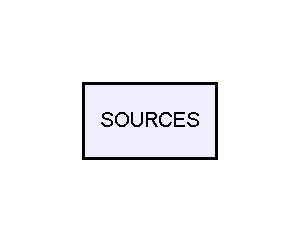
\includegraphics[width=144pt]{dir_f954d619dd741ca6dd310b84cdef7dac_dep}
\end{center}
\end{figure}
\subsection*{Files}
\begin{DoxyCompactItemize}
\item 
file \hyperlink{ALGEBRA_8f90}{ALGEBRA.f90}
\item 
file \hyperlink{DATATYPES_8f90}{DATATYPES.f90}
\item 
file \hyperlink{FFT_8F}{FFT.F}
\item 
file \hyperlink{INIT_8f90}{INIT.f90}
\item 
file \hyperlink{IO_8f90}{IO.f90}
\item 
file \hyperlink{ONERROR_8f90}{ONERROR.f90}
\item 
file \hyperlink{PREMIXED_8f90}{PREMIXED.f90}
\item 
file \hyperlink{SPECTRAL__ANALYSIS_8f90}{SPECTRAL\_\-ANALYSIS.f90}
\item 
file \hyperlink{STATISTICS_8f90}{STATISTICS.f90}
\item 
file \hyperlink{TIMER_8f90}{TIMER.f90}
\end{DoxyCompactItemize}

\chapter{Module Documentation}
\hypertarget{namespaceFIELD__CLASS}{
\section{FIELD\_\-CLASS Module Reference}
\label{namespaceFIELD__CLASS}\index{FIELD\_\-CLASS@{FIELD\_\-CLASS}}
}
\subsection*{Data Types}
\begin{DoxyCompactItemize}
\item 
type \hyperlink{typeFIELD__CLASS_1_1field}{field}
\end{DoxyCompactItemize}

\hypertarget{namespaceINIT}{
\section{INIT Module Reference}
\label{namespaceINIT}\index{INIT@{INIT}}
}


Defines some user specified input parameters.  


\subsection*{Variables}
\begin{DoxyCompactItemize}
\item 
INTEGER(SP) \hyperlink{namespaceINIT_a0220cec3830356e24c2d71461783251b}{DIM}
\item 
REAL(DP) \hyperlink{namespaceINIT_a2408b167edb7d420e8c30e9844d9f657}{DX}
\end{DoxyCompactItemize}


\subsection{Detailed Description}
Defines some user specified input parameters. \begin{DoxyAuthor}{Author}
Felix Dietzsch 
\end{DoxyAuthor}


\subsection{Variable Documentation}
\hypertarget{namespaceINIT_a0220cec3830356e24c2d71461783251b}{
\index{INIT@{INIT}!DIM@{DIM}}
\index{DIM@{DIM}!INIT@{INIT}}
\subsubsection[{DIM}]{\setlength{\rightskip}{0pt plus 5cm}INTEGER(SP) {\bf INIT::DIM}}}
\label{namespaceINIT_a0220cec3830356e24c2d71461783251b}


Definition at line 15 of file INIT.f90.



Referenced by SPECTRAL\_\-ANALYSIS().

\hypertarget{namespaceINIT_a2408b167edb7d420e8c30e9844d9f657}{
\index{INIT@{INIT}!DX@{DX}}
\index{DX@{DX}!INIT@{INIT}}
\subsubsection[{DX}]{\setlength{\rightskip}{0pt plus 5cm}REAL(DP) {\bf INIT::DX}}}
\label{namespaceINIT_a2408b167edb7d420e8c30e9844d9f657}


Definition at line 16 of file INIT.f90.


\hypertarget{namespaceIO__CLASS}{
\section{IO\_\-CLASS Module Reference}
\label{namespaceIO__CLASS}\index{IO\_\-CLASS@{IO\_\-CLASS}}
}


Controls the input and output for the underlying postprocessor.  


\subsection*{Data Types}
\begin{DoxyCompactItemize}
\item 
interface \hyperlink{interfaceIO__CLASS_1_1INDEXING}{INDEXING}
\item 
interface \hyperlink{interfaceIO__CLASS_1_1READCOORD}{READCOORD}
\item 
interface \hyperlink{interfaceIO__CLASS_1_1READ__DIM}{READ\_\-DIM}
\item 
interface \hyperlink{interfaceIO__CLASS_1_1READ__GRID}{READ\_\-GRID}
\item 
interface \hyperlink{interfaceIO__CLASS_1_1READVALUE}{READVALUE}
\item 
interface \hyperlink{interfaceIO__CLASS_1_1WRITE__TEMPER}{WRITE\_\-TEMPER}
\item 
interface \hyperlink{interfaceIO__CLASS_1_1WRITE__PROG}{WRITE\_\-PROG}
\item 
interface \hyperlink{interfaceIO__CLASS_1_1READVEL}{READVEL}
\item 
interface \hyperlink{interfaceIO__CLASS_1_1READVEL__BIN}{READVEL\_\-BIN}
\item 
type \hyperlink{typeIO__CLASS_1_1IO}{IO}
\end{DoxyCompactItemize}
\subsection*{Functions/Subroutines}
\begin{DoxyCompactItemize}
\item 
subroutine \hyperlink{namespaceIO__CLASS_afb3b43393c81d05f437ae1359acf77d2}{read\_\-dummy\_\-sub} (this, filename, dimen)
\item 
REAL(DP), dimension(:,:), pointer \hyperlink{namespaceIO__CLASS_a9fd49cecb24a51f12650f5249285c05f}{field\_\-f} (this)
\item 
REAL \hyperlink{namespaceIO__CLASS_a16514873e600c2fbfde6897a92c88d5e}{number\_\-of\_\-nodes\_\-x\_\-f} (this)
\item 
REAL \hyperlink{namespaceIO__CLASS_a67cf6d63ec2af6429ed8ef6885ac143a}{number\_\-of\_\-nodes\_\-y\_\-f} (this)
\item 
REAL \hyperlink{namespaceIO__CLASS_aa9b327cdca2173b0269ec5007a8ab9f1}{number\_\-of\_\-nodes\_\-z\_\-f} (this)
\end{DoxyCompactItemize}


\subsection{Detailed Description}
Controls the input and output for the underlying postprocessor. \begin{DoxyAuthor}{Author}
Felix Dietzsch 
\end{DoxyAuthor}


\subsection{Function/Subroutine Documentation}
\hypertarget{namespaceIO__CLASS_a9fd49cecb24a51f12650f5249285c05f}{
\index{IO\_\-CLASS@{IO\_\-CLASS}!field\_\-f@{field\_\-f}}
\index{field\_\-f@{field\_\-f}!IO_CLASS@{IO\_\-CLASS}}
\subsubsection[{field\_\-f}]{\setlength{\rightskip}{0pt plus 5cm}REAL(DP),dimension(:,:),pointer IO\_\-CLASS::field\_\-f (
\begin{DoxyParamCaption}
\item[{CLASS(IO)}]{this}
\end{DoxyParamCaption}
)}}
\label{namespaceIO__CLASS_a9fd49cecb24a51f12650f5249285c05f}


Definition at line 241 of file IO.f90.



Referenced by IO\_\-CLASS::IO::field().

\hypertarget{namespaceIO__CLASS_a16514873e600c2fbfde6897a92c88d5e}{
\index{IO\_\-CLASS@{IO\_\-CLASS}!number\_\-of\_\-nodes\_\-x\_\-f@{number\_\-of\_\-nodes\_\-x\_\-f}}
\index{number\_\-of\_\-nodes\_\-x\_\-f@{number\_\-of\_\-nodes\_\-x\_\-f}!IO_CLASS@{IO\_\-CLASS}}
\subsubsection[{number\_\-of\_\-nodes\_\-x\_\-f}]{\setlength{\rightskip}{0pt plus 5cm}REAL IO\_\-CLASS::number\_\-of\_\-nodes\_\-x\_\-f (
\begin{DoxyParamCaption}
\item[{CLASS(IO)}]{this}
\end{DoxyParamCaption}
)}}
\label{namespaceIO__CLASS_a16514873e600c2fbfde6897a92c88d5e}


Definition at line 261 of file IO.f90.



Referenced by IO\_\-CLASS::IO::NX().

\hypertarget{namespaceIO__CLASS_a67cf6d63ec2af6429ed8ef6885ac143a}{
\index{IO\_\-CLASS@{IO\_\-CLASS}!number\_\-of\_\-nodes\_\-y\_\-f@{number\_\-of\_\-nodes\_\-y\_\-f}}
\index{number\_\-of\_\-nodes\_\-y\_\-f@{number\_\-of\_\-nodes\_\-y\_\-f}!IO_CLASS@{IO\_\-CLASS}}
\subsubsection[{number\_\-of\_\-nodes\_\-y\_\-f}]{\setlength{\rightskip}{0pt plus 5cm}REAL IO\_\-CLASS::number\_\-of\_\-nodes\_\-y\_\-f (
\begin{DoxyParamCaption}
\item[{CLASS(IO)}]{this}
\end{DoxyParamCaption}
)}}
\label{namespaceIO__CLASS_a67cf6d63ec2af6429ed8ef6885ac143a}


Definition at line 267 of file IO.f90.



Referenced by IO\_\-CLASS::IO::NY().

\hypertarget{namespaceIO__CLASS_aa9b327cdca2173b0269ec5007a8ab9f1}{
\index{IO\_\-CLASS@{IO\_\-CLASS}!number\_\-of\_\-nodes\_\-z\_\-f@{number\_\-of\_\-nodes\_\-z\_\-f}}
\index{number\_\-of\_\-nodes\_\-z\_\-f@{number\_\-of\_\-nodes\_\-z\_\-f}!IO_CLASS@{IO\_\-CLASS}}
\subsubsection[{number\_\-of\_\-nodes\_\-z\_\-f}]{\setlength{\rightskip}{0pt plus 5cm}REAL IO\_\-CLASS::number\_\-of\_\-nodes\_\-z\_\-f (
\begin{DoxyParamCaption}
\item[{CLASS(IO)}]{this}
\end{DoxyParamCaption}
)}}
\label{namespaceIO__CLASS_aa9b327cdca2173b0269ec5007a8ab9f1}


Definition at line 273 of file IO.f90.



Referenced by IO\_\-CLASS::IO::NZ().

\hypertarget{namespaceIO__CLASS_afb3b43393c81d05f437ae1359acf77d2}{
\index{IO\_\-CLASS@{IO\_\-CLASS}!read\_\-dummy\_\-sub@{read\_\-dummy\_\-sub}}
\index{read\_\-dummy\_\-sub@{read\_\-dummy\_\-sub}!IO_CLASS@{IO\_\-CLASS}}
\subsubsection[{read\_\-dummy\_\-sub}]{\setlength{\rightskip}{0pt plus 5cm}subroutine IO\_\-CLASS::read\_\-dummy\_\-sub (
\begin{DoxyParamCaption}
\item[{CLASS(IO)}]{this, }
\item[{CHARACTER(LEN=$\ast$),intent(in)}]{filename, }
\item[{INTEGER(SP)}]{dimen}
\end{DoxyParamCaption}
)}}
\label{namespaceIO__CLASS_afb3b43393c81d05f437ae1359acf77d2}


Definition at line 164 of file IO.f90.



Referenced by IO\_\-CLASS::IO::read\_\-file().


\hypertarget{namespaceNRTYPE}{
\section{NRTYPE Module Reference}
\label{namespaceNRTYPE}\index{NRTYPE@{NRTYPE}}
}


Defines some basic kinds for variable definitions.  


\subsection*{Variables}
\begin{DoxyCompactItemize}
\item 
INTEGER, parameter \hyperlink{namespaceNRTYPE_a203d15b0d754eb809bb2d9689c0f4a20}{SPC} = KIND((1.0, 1.0))
\item 
INTEGER, parameter \hyperlink{namespaceNRTYPE_aef0a8a355687c7f4bb0cfc4da1fa7dc1}{DPC} = KIND((1.0D0, 1.0D0))
\item 
INTEGER, parameter \hyperlink{namespaceNRTYPE_a0e27dcc6c8b8c3b676b0ebdeda77f849}{SP} = KIND(1.0)
\item 
INTEGER, parameter \hyperlink{namespaceNRTYPE_ac04234d0d9fbb992bc90e09d33317d5a}{DP} = KIND(1.0D0)
\item 
INTEGER, parameter \hyperlink{namespaceNRTYPE_a58a56fb59c61ae4e8af28eabfe3d3b59}{I4B} = SELECTED\_\-INT\_\-KIND(R=9)
\item 
INTEGER, parameter \hyperlink{namespaceNRTYPE_ac467681e919a8be9d83a8bf1808d497c}{LGT} = KIND(.true.)
\item 
REAL(\hyperlink{namespaceNRTYPE_ac04234d0d9fbb992bc90e09d33317d5a}{DP}), parameter \hyperlink{namespaceNRTYPE_a651a3a781cff22a0a0886657381949db}{PI\_\-D} = 3.141592653589793238462643383279502884197\_\-dp
\item 
REAL(\hyperlink{namespaceNRTYPE_ac04234d0d9fbb992bc90e09d33317d5a}{DP}), parameter \hyperlink{namespaceNRTYPE_a39b7abf71e8b2487187ea1b1f3a2dedf}{TWOPI\_\-D} = 6.283185307179586476925286766559005768394\_\-dp
\end{DoxyCompactItemize}


\subsection{Detailed Description}
Defines some basic kinds for variable definitions. \begin{DoxyAuthor}{Author}
Felix Dietzsch
\end{DoxyAuthor}
Defines some basic kinds for variable definitions. It is strongly recommended to use this module in every module to be defined. 

\subsection{Variable Documentation}
\hypertarget{namespaceNRTYPE_ac04234d0d9fbb992bc90e09d33317d5a}{
\index{NRTYPE@{NRTYPE}!DP@{DP}}
\index{DP@{DP}!NRTYPE@{NRTYPE}}
\subsubsection[{DP}]{\setlength{\rightskip}{0pt plus 5cm}INTEGER,parameter {\bf NRTYPE::DP} = KIND(1.0D0)}}
\label{namespaceNRTYPE_ac04234d0d9fbb992bc90e09d33317d5a}


Definition at line 20 of file DATATYPES.f90.

\hypertarget{namespaceNRTYPE_aef0a8a355687c7f4bb0cfc4da1fa7dc1}{
\index{NRTYPE@{NRTYPE}!DPC@{DPC}}
\index{DPC@{DPC}!NRTYPE@{NRTYPE}}
\subsubsection[{DPC}]{\setlength{\rightskip}{0pt plus 5cm}INTEGER,parameter {\bf NRTYPE::DPC} = KIND((1.0D0, 1.0D0))}}
\label{namespaceNRTYPE_aef0a8a355687c7f4bb0cfc4da1fa7dc1}


Definition at line 18 of file DATATYPES.f90.

\hypertarget{namespaceNRTYPE_a58a56fb59c61ae4e8af28eabfe3d3b59}{
\index{NRTYPE@{NRTYPE}!I4B@{I4B}}
\index{I4B@{I4B}!NRTYPE@{NRTYPE}}
\subsubsection[{I4B}]{\setlength{\rightskip}{0pt plus 5cm}INTEGER,parameter {\bf NRTYPE::I4B} = SELECTED\_\-INT\_\-KIND(R=9)}}
\label{namespaceNRTYPE_a58a56fb59c61ae4e8af28eabfe3d3b59}


Definition at line 21 of file DATATYPES.f90.

\hypertarget{namespaceNRTYPE_ac467681e919a8be9d83a8bf1808d497c}{
\index{NRTYPE@{NRTYPE}!LGT@{LGT}}
\index{LGT@{LGT}!NRTYPE@{NRTYPE}}
\subsubsection[{LGT}]{\setlength{\rightskip}{0pt plus 5cm}INTEGER,parameter {\bf NRTYPE::LGT} = KIND(.true.)}}
\label{namespaceNRTYPE_ac467681e919a8be9d83a8bf1808d497c}


Definition at line 22 of file DATATYPES.f90.

\hypertarget{namespaceNRTYPE_a651a3a781cff22a0a0886657381949db}{
\index{NRTYPE@{NRTYPE}!PI\_\-D@{PI\_\-D}}
\index{PI\_\-D@{PI\_\-D}!NRTYPE@{NRTYPE}}
\subsubsection[{PI\_\-D}]{\setlength{\rightskip}{0pt plus 5cm}REAL({\bf DP}),parameter {\bf NRTYPE::PI\_\-D} = 3.141592653589793238462643383279502884197\_\-dp}}
\label{namespaceNRTYPE_a651a3a781cff22a0a0886657381949db}


Definition at line 23 of file DATATYPES.f90.

\hypertarget{namespaceNRTYPE_a0e27dcc6c8b8c3b676b0ebdeda77f849}{
\index{NRTYPE@{NRTYPE}!SP@{SP}}
\index{SP@{SP}!NRTYPE@{NRTYPE}}
\subsubsection[{SP}]{\setlength{\rightskip}{0pt plus 5cm}INTEGER,parameter {\bf NRTYPE::SP} = KIND(1.0)}}
\label{namespaceNRTYPE_a0e27dcc6c8b8c3b676b0ebdeda77f849}


Definition at line 19 of file DATATYPES.f90.

\hypertarget{namespaceNRTYPE_a203d15b0d754eb809bb2d9689c0f4a20}{
\index{NRTYPE@{NRTYPE}!SPC@{SPC}}
\index{SPC@{SPC}!NRTYPE@{NRTYPE}}
\subsubsection[{SPC}]{\setlength{\rightskip}{0pt plus 5cm}INTEGER,parameter {\bf NRTYPE::SPC} = KIND((1.0, 1.0))}}
\label{namespaceNRTYPE_a203d15b0d754eb809bb2d9689c0f4a20}


Definition at line 17 of file DATATYPES.f90.

\hypertarget{namespaceNRTYPE_a39b7abf71e8b2487187ea1b1f3a2dedf}{
\index{NRTYPE@{NRTYPE}!TWOPI\_\-D@{TWOPI\_\-D}}
\index{TWOPI\_\-D@{TWOPI\_\-D}!NRTYPE@{NRTYPE}}
\subsubsection[{TWOPI\_\-D}]{\setlength{\rightskip}{0pt plus 5cm}REAL({\bf DP}),parameter {\bf NRTYPE::TWOPI\_\-D} = 6.283185307179586476925286766559005768394\_\-dp}}
\label{namespaceNRTYPE_a39b7abf71e8b2487187ea1b1f3a2dedf}


Definition at line 24 of file DATATYPES.f90.


\hypertarget{namespaceONERROR}{
\section{ONERROR Module Reference}
\label{namespaceONERROR}\index{ONERROR@{ONERROR}}
}


Contains definition of error messages.  


\subsection*{Functions/Subroutines}
\begin{DoxyCompactItemize}
\item 
subroutine \hyperlink{namespaceONERROR_a886bc1a5bcf6a0b449daef743c63ca96}{ALLOCATION\_\-ERROR} (IERR)
\begin{DoxyCompactList}\small\item\em Prints allocation error message. \end{DoxyCompactList}\item 
subroutine \hyperlink{namespaceONERROR_a65114034ce76f426e610df6aa8c4e69b}{DEALLOCATION\_\-ERROR} (IERR, UNIT\_\-VALUE)
\begin{DoxyCompactList}\small\item\em Prints deallocation error message. \end{DoxyCompactList}\end{DoxyCompactItemize}


\subsection{Detailed Description}
Contains definition of error messages. \begin{DoxyAuthor}{Author}
Felix Dietzsch 
\end{DoxyAuthor}


\subsection{Function/Subroutine Documentation}
\hypertarget{namespaceONERROR_a886bc1a5bcf6a0b449daef743c63ca96}{
\index{ONERROR@{ONERROR}!ALLOCATION\_\-ERROR@{ALLOCATION\_\-ERROR}}
\index{ALLOCATION\_\-ERROR@{ALLOCATION\_\-ERROR}!ONERROR@{ONERROR}}
\subsubsection[{ALLOCATION\_\-ERROR}]{\setlength{\rightskip}{0pt plus 5cm}subroutine ONERROR::ALLOCATION\_\-ERROR (
\begin{DoxyParamCaption}
\item[{INTEGER}]{IERR}
\end{DoxyParamCaption}
)}}
\label{namespaceONERROR_a886bc1a5bcf6a0b449daef743c63ca96}


Prints allocation error message. 

\begin{DoxyAuthor}{Author}
Felix Dietzsch 
\end{DoxyAuthor}

\begin{DoxyParams}[1]{Parameters}
\mbox{\tt in}  & {\em IERR} & Error descriptor \\
\hline
\end{DoxyParams}


Definition at line 28 of file ONERROR.f90.



Referenced by SPECTRAL\_\-ANALYSIS().

\hypertarget{namespaceONERROR_a65114034ce76f426e610df6aa8c4e69b}{
\index{ONERROR@{ONERROR}!DEALLOCATION\_\-ERROR@{DEALLOCATION\_\-ERROR}}
\index{DEALLOCATION\_\-ERROR@{DEALLOCATION\_\-ERROR}!ONERROR@{ONERROR}}
\subsubsection[{DEALLOCATION\_\-ERROR}]{\setlength{\rightskip}{0pt plus 5cm}subroutine ONERROR::DEALLOCATION\_\-ERROR (
\begin{DoxyParamCaption}
\item[{INTEGER}]{IERR, }
\item[{INTEGER}]{UNIT\_\-VALUE}
\end{DoxyParamCaption}
)}}
\label{namespaceONERROR_a65114034ce76f426e610df6aa8c4e69b}


Prints deallocation error message. 

\begin{DoxyAuthor}{Author}
Felix Dietzsch 
\end{DoxyAuthor}

\begin{DoxyParams}[1]{Parameters}
\mbox{\tt in}  & {\em IERR} & Error descriptor \\
\hline
\mbox{\tt in}  & {\em UNIT\_\-VALUE} & Error descriptor\par
 1 -\/-\/ COORD\par
 2 -\/-\/ INDX\par
 3 -\/-\/ INDY\par
 4 -\/-\/ INDZ\par
 5 -\/-\/ UUX\par
 6 -\/-\/ UUY\par
 7 -\/-\/ UUZ\par
 \\
\hline
\end{DoxyParams}


Definition at line 53 of file ONERROR.f90.


\hypertarget{namespacePREMIXED__CLASS}{
\section{PREMIXED\_\-CLASS Module Reference}
\label{namespacePREMIXED__CLASS}\index{PREMIXED\_\-CLASS@{PREMIXED\_\-CLASS}}
}
\subsection*{Data Types}
\begin{DoxyCompactItemize}
\item 
interface \hyperlink{interfacePREMIXED__CLASS_1_1COMP__PROGRESS}{COMP\_\-PROGRESS}
\end{DoxyCompactItemize}
\subsection*{Functions/Subroutines}
\begin{DoxyCompactItemize}
\item 
subroutine \hyperlink{namespacePREMIXED__CLASS_a8e8fde9973a06836544f2e0171177fff}{COMP\_\-PROGRESS} (TEMPER, PROG\_\-VAR, SPEC, SPECUB, SPECB, SAVEVAR)
\end{DoxyCompactItemize}


\subsection{Function/Subroutine Documentation}
\hypertarget{namespacePREMIXED__CLASS_a8e8fde9973a06836544f2e0171177fff}{
\index{PREMIXED\_\-CLASS@{PREMIXED\_\-CLASS}!COMP\_\-PROGRESS@{COMP\_\-PROGRESS}}
\index{COMP\_\-PROGRESS@{COMP\_\-PROGRESS}!PREMIXED_CLASS@{PREMIXED\_\-CLASS}}
\subsubsection[{COMP\_\-PROGRESS}]{\setlength{\rightskip}{0pt plus 5cm}subroutine {\bf PREMIXED\_\-CLASS::COMP\_\-PROGRESS} (
\begin{DoxyParamCaption}
\item[{REAL(DP),dimension(:,:,:),intent(in)}]{TEMPER, }
\item[{REAL(DP),dimension(:,:,:),intent(inout)}]{PROG\_\-VAR, }
\item[{REAL(DP),dimension(:,:,:),intent(in),optional}]{SPEC, }
\item[{REAL(DP),intent(in),optional}]{SPECUB, }
\item[{REAL(DP),intent(in),optional}]{SPECB, }
\item[{LOGICAL,intent(in),optional}]{SAVEVAR}
\end{DoxyParamCaption}
)}}
\label{namespacePREMIXED__CLASS_a8e8fde9973a06836544f2e0171177fff}


Definition at line 7 of file PREMIXED.f90.


\hypertarget{namespaceSTATISTICS}{
\section{STATISTICS Module Reference}
\label{namespaceSTATISTICS}\index{STATISTICS@{STATISTICS}}
}


Provides functions for statistical computations.  


\subsection*{Data Types}
\begin{DoxyCompactItemize}
\item 
interface \hyperlink{interfaceSTATISTICS_1_1MEAN}{MEAN}
\item 
interface \hyperlink{interfaceSTATISTICS_1_1CORREL}{CORREL}
\item 
interface \hyperlink{interfaceSTATISTICS_1_1SHIFT}{SHIFT}
\item 
interface \hyperlink{interfaceSTATISTICS_1_1SPECTR}{SPECTR}
\item 
interface \hyperlink{interfaceSTATISTICS_1_1DEVIAT}{DEVIAT}
\end{DoxyCompactItemize}
\subsection*{Functions/Subroutines}
\begin{DoxyCompactItemize}
\item 
subroutine \hyperlink{namespaceSTATISTICS_a4a3e7e4d1eb020e1128c01e60da55ead}{SPEC2D} (IN1, IN2, NX, NY, OUT)
\begin{DoxyCompactList}\small\item\em Computes the three dimensional energy spectrum as the fourier transformation\par
 of the auto-\/correlation function. In the first step all three velocity\par
 components are fourier transformed. The second step consists of multiplying\par
 each transform with its conjugate complex in order to get the elements of the\par
 main diagonal of the velocity spectrum tensor \[\hat{R}_{ii}\left(\kappa,t\right)= \left<\hat{u}_i^{*}\left(\kappa,t\right)\,\hat{u}_i\left(\kappa,t\right)\right>= \Phi_{ii}\left(\kappa,t\right).\] After the components of $\Phi$ have been determined an integration over\par
 spherical shells has to be computed in order to get the three dimensional\par
 velocity spectrum. \[ E(k)=\oint\frac{1}{2}\Phi_{ii}(\kappa)\,d\mathrm{S}(\kappa) \] \end{DoxyCompactList}\item 
subroutine \hyperlink{namespaceSTATISTICS_abb792b2e62e57165b7e93764e07d1100}{SPEC3D} (PROCNUM, IN1, IN2, IN3, NX, NY, NZ, OUT)
\begin{DoxyCompactList}\small\item\em Computes the three dimensional energy spectrum as the fourier transformation\par
 of the auto-\/correlation function. In the first step all three velocity\par
 components are fourier transformed. The second step consists of multiplying\par
 each transform with its conjugate complex in order to get the elements of the\par
 main diagonal of the velocity spectrum tensor \[\hat{R}_{ii}\left(\kappa,t\right)= \left<\hat{u}_i^{*}\left(\kappa,t\right)\,\hat{u}_i\left(\kappa,t\right)\right>= \Phi_{ii}\left(\kappa,t\right).\] After the components of $\Phi$ have been determined an integration over\par
 spherical shells has to be computed in order to get the three dimensional\par
 velocity spectrum. \[ E(k)=\oint\frac{1}{2}\Phi_{ii}(\kappa)\,d\mathrm{S}(\kappa) \] \end{DoxyCompactList}\item 
subroutine \hyperlink{namespaceSTATISTICS_a96f2830bd74ef7e612bb9b567a488fcb}{DEVIATION} (VELO, NX, NY, NZ, SIGMA)
\begin{DoxyCompactList}\small\item\em Computes the standard deviation of the 3D input array. It is computed according to \[\sigma = \sqrt{\frac{1}{N} \sum_{i=1}^N (x_i - \mu)^2}, {\rm \ \ where\ \ } \mu = \frac{1}{N} \sum_{i=1}^N x_i. \] \end{DoxyCompactList}\item 
subroutine \hyperlink{namespaceSTATISTICS_ac51d5b789da17893b95107ddcb97813f}{FFTSHIFT} (IN, NX, NY)
\begin{DoxyCompactList}\small\item\em Shifts the input array towards the zero frequencies. \end{DoxyCompactList}\item 
subroutine \hyperlink{namespaceSTATISTICS_a6631e38a843e8bfa986d426daebd6f4c}{CORREL3D} (IN, NX, NY, NZ, OUT)
\begin{DoxyCompactList}\small\item\em Computes the auto-\/correlation coefficients of the 3D input array. The general definition of the auto-\/correlation (often exressed as the covariance) function is \[\mathrm{cov}(f,f)=\left(f\star f\right)(r)=\int_0^{\infty}f(x)\,f(x+r)\,dx \] One important feature of the correlation function is that is satisfies \[\mathcal{F}\{f\star f\}=(\mathcal{F}\{f\})^*\cdot\mathcal{F}\{f\}. \] In the code this allows for fast computations of the correlation function using the FFT approach. In order to get the correlation coefficients, the previously mentioned function has to be devided by standard deviations of the input arrays. \[r=\frac{\mathrm{cov}(f,f)}{\sigma_f\,\sigma_f} \] \end{DoxyCompactList}\item 
subroutine \hyperlink{namespaceSTATISTICS_a2529efc59bb06c5f2280df7277bf5c7d}{XCORREL} (IN1, IN2, NX, NY, NZ, OUT)
\begin{DoxyCompactList}\small\item\em Computes the cross-\/correlation coefficients of the 3D input arrays. The general definition of the cross-\/correlation (often exressed as the covariance) function is \[\mathrm{cov}(f,g)=\left(f\star g\right)(r)=\int_0^{\infty}f(x)\,g(x+r)\,dx \] One important feature of the correlation function is that is satisfies \[\mathcal{F}\{f\star g\}=(\mathcal{F}\{f\})^*\cdot\mathcal{F}\{g\}. \] In the code this allows for fast computations of the correlation function using the FFT approach. In order to get the correlation coefficients, the previously mentioned function has to be devided by standard deviations of the input arrays. \[r=\frac{\mathrm{cov}(f,g)}{\sigma_f\,\sigma_g} \] Computes the cross-\/correlation of the 3D input array \end{DoxyCompactList}\item 
subroutine \hyperlink{namespaceSTATISTICS_a0e5d171eb0600a926c45883d16628bc5}{MEAN1D} (M, NX)
\item 
subroutine \hyperlink{namespaceSTATISTICS_a95b82ef7e03a03d4b2ff850710558843}{MEAN3D} (M, NX, NY, NZ, \hyperlink{interfaceSTATISTICS_1_1MEAN}{MEAN})
\begin{DoxyCompactList}\small\item\em Shifts the input array towards the zero frequencies. \end{DoxyCompactList}\item 
subroutine \hyperlink{namespaceSTATISTICS_a2e2608ba8eefb8af3541e4e9a09a6482}{MEAN4D} (M, NX, NY, NZ, DIM, \hyperlink{interfaceSTATISTICS_1_1MEAN}{MEAN})
\end{DoxyCompactItemize}


\subsection{Detailed Description}
Provides functions for statistical computations. \begin{DoxyAuthor}{Author}
Felix Dietzsch 
\end{DoxyAuthor}


\subsection{Function/Subroutine Documentation}
\hypertarget{namespaceSTATISTICS_a6631e38a843e8bfa986d426daebd6f4c}{
\index{STATISTICS@{STATISTICS}!CORREL3D@{CORREL3D}}
\index{CORREL3D@{CORREL3D}!STATISTICS@{STATISTICS}}
\subsubsection[{CORREL3D}]{\setlength{\rightskip}{0pt plus 5cm}subroutine STATISTICS::CORREL3D (
\begin{DoxyParamCaption}
\item[{COMPLEX(DPC),dimension(:,:,:),intent(in)}]{IN, }
\item[{INTEGER(SP)}]{NX, }
\item[{INTEGER(SP)}]{NY, }
\item[{INTEGER(SP)}]{NZ, }
\item[{COMPLEX(DPC),dimension(:,:,:),intent(inout)}]{OUT}
\end{DoxyParamCaption}
)}}
\label{namespaceSTATISTICS_a6631e38a843e8bfa986d426daebd6f4c}


Computes the auto-\/correlation coefficients of the 3D input array. The general definition of the auto-\/correlation (often exressed as the covariance) function is \[\mathrm{cov}(f,f)=\left(f\star f\right)(r)=\int_0^{\infty}f(x)\,f(x+r)\,dx \] One important feature of the correlation function is that is satisfies \[\mathcal{F}\{f\star f\}=(\mathcal{F}\{f\})^*\cdot\mathcal{F}\{f\}. \] In the code this allows for fast computations of the correlation function using the FFT approach. In order to get the correlation coefficients, the previously mentioned function has to be devided by standard deviations of the input arrays. \[r=\frac{\mathrm{cov}(f,f)}{\sigma_f\,\sigma_f} \] 

\begin{DoxyAuthor}{Author}
Felix Dietzsch Computes the auto-\/correlation coefficients of the 3D input array 
\end{DoxyAuthor}

\begin{DoxyParams}[1]{Parameters}
\mbox{\tt in}  & {\em IN} & 3D array for the computation of the 3D auto-\/correlation coefficients \\
\hline
\mbox{\tt in}  & {\em NX} & Number of nodes in x direction \\
\hline
\mbox{\tt in}  & {\em NY} & Number of nodes in y direction \\
\hline
\mbox{\tt in}  & {\em NZ} & Number of nodes in z direction \\
\hline
\mbox{\tt out}  & {\em OUT} & 3D array of auto-\/correlation coeffcients \\
\hline
\end{DoxyParams}


Definition at line 416 of file STATISTICS.f90.



References DEVIATION().



Here is the call graph for this function:\nopagebreak
\begin{figure}[H]
\begin{center}
\leavevmode
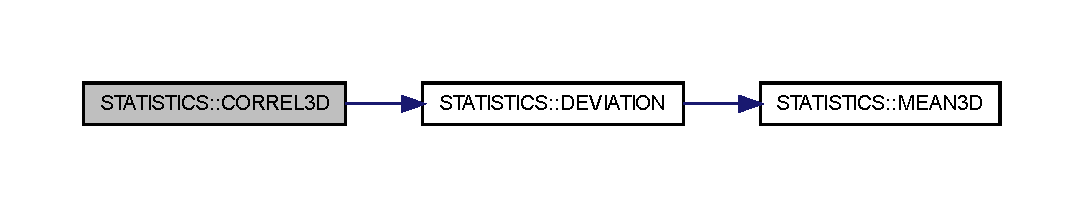
\includegraphics[width=400pt]{namespaceSTATISTICS_a6631e38a843e8bfa986d426daebd6f4c_cgraph}
\end{center}
\end{figure}


\hypertarget{namespaceSTATISTICS_a96f2830bd74ef7e612bb9b567a488fcb}{
\index{STATISTICS@{STATISTICS}!DEVIATION@{DEVIATION}}
\index{DEVIATION@{DEVIATION}!STATISTICS@{STATISTICS}}
\subsubsection[{DEVIATION}]{\setlength{\rightskip}{0pt plus 5cm}subroutine STATISTICS::DEVIATION (
\begin{DoxyParamCaption}
\item[{REAL(DP),dimension(:,:,:)}]{VELO, }
\item[{INTEGER(SP)}]{NX, }
\item[{INTEGER(SP)}]{NY, }
\item[{}]{NZ, }
\item[{REAL(DP)}]{SIGMA}
\end{DoxyParamCaption}
)}}
\label{namespaceSTATISTICS_a96f2830bd74ef7e612bb9b567a488fcb}


Computes the standard deviation of the 3D input array. It is computed according to \[\sigma = \sqrt{\frac{1}{N} \sum_{i=1}^N (x_i - \mu)^2}, {\rm \ \ where\ \ } \mu = \frac{1}{N} \sum_{i=1}^N x_i. \] 

\begin{DoxyAuthor}{Author}
Felix Dietzsch Computes the standard deviation of the 3D input array. 
\end{DoxyAuthor}

\begin{DoxyParams}[1]{Parameters}
\mbox{\tt in}  & {\em VELO} & 3D array of which the deviation is to be computed \\
\hline
\mbox{\tt in}  & {\em NX} & Number of nodes in x direction \\
\hline
\mbox{\tt in}  & {\em NY} & Number of nodes in y direction \\
\hline
\mbox{\tt in}  & {\em NZ} & Number of nodes in z direction \\
\hline
\mbox{\tt out}  & {\em SIGMA} & Standard deviation of the input array velocities \\
\hline
\end{DoxyParams}


Definition at line 319 of file STATISTICS.f90.



References MEAN3D().



Referenced by CORREL3D(), and XCORREL().



Here is the call graph for this function:\nopagebreak
\begin{figure}[H]
\begin{center}
\leavevmode
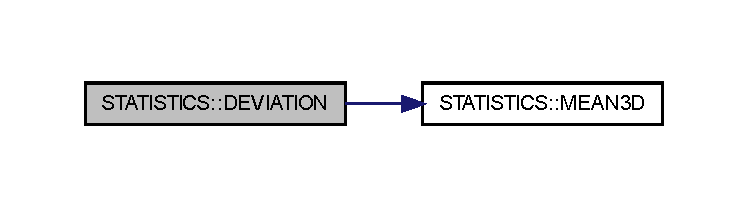
\includegraphics[width=358pt]{namespaceSTATISTICS_a96f2830bd74ef7e612bb9b567a488fcb_cgraph}
\end{center}
\end{figure}


\hypertarget{namespaceSTATISTICS_ac51d5b789da17893b95107ddcb97813f}{
\index{STATISTICS@{STATISTICS}!FFTSHIFT@{FFTSHIFT}}
\index{FFTSHIFT@{FFTSHIFT}!STATISTICS@{STATISTICS}}
\subsubsection[{FFTSHIFT}]{\setlength{\rightskip}{0pt plus 5cm}subroutine STATISTICS::FFTSHIFT (
\begin{DoxyParamCaption}
\item[{COMPLEX(DPC),dimension(nx,ny),intent(inout)}]{IN, }
\item[{INTEGER(SP)}]{NX, }
\item[{INTEGER(SP)}]{NY}
\end{DoxyParamCaption}
)}}
\label{namespaceSTATISTICS_ac51d5b789da17893b95107ddcb97813f}


Shifts the input array towards the zero frequencies. 

\begin{DoxyAuthor}{Author}
Felix Dietzsch  Shifts the input array towards the zero frequencies. 
\end{DoxyAuthor}

\begin{DoxyParams}[1]{Parameters}
\mbox{\tt in}  & {\em IN} & 2D array of shifted frequencies \\
\hline
\mbox{\tt in}  & {\em NX} & Number of nodes in y direction \\
\hline
\mbox{\tt in}  & {\em NY} & Number of nodes in z direction \\
\hline
\mbox{\tt out}  & {\em IN} & 2D array of shifted frequencies \\
\hline
\end{DoxyParams}


Definition at line 362 of file STATISTICS.f90.

\hypertarget{namespaceSTATISTICS_a0e5d171eb0600a926c45883d16628bc5}{
\index{STATISTICS@{STATISTICS}!MEAN1D@{MEAN1D}}
\index{MEAN1D@{MEAN1D}!STATISTICS@{STATISTICS}}
\subsubsection[{MEAN1D}]{\setlength{\rightskip}{0pt plus 5cm}subroutine STATISTICS::MEAN1D (
\begin{DoxyParamCaption}
\item[{REAL(DP),dimension(:)}]{M, }
\item[{INTEGER(SP)}]{NX}
\end{DoxyParamCaption}
)}}
\label{namespaceSTATISTICS_a0e5d171eb0600a926c45883d16628bc5}


Definition at line 526 of file STATISTICS.f90.

\hypertarget{namespaceSTATISTICS_a95b82ef7e03a03d4b2ff850710558843}{
\index{STATISTICS@{STATISTICS}!MEAN3D@{MEAN3D}}
\index{MEAN3D@{MEAN3D}!STATISTICS@{STATISTICS}}
\subsubsection[{MEAN3D}]{\setlength{\rightskip}{0pt plus 5cm}subroutine STATISTICS::MEAN3D (
\begin{DoxyParamCaption}
\item[{REAL(DP),dimension(:,:,:)}]{M, }
\item[{INTEGER(SP)}]{NX, }
\item[{INTEGER(SP)}]{NY, }
\item[{}]{NZ, }
\item[{REAL(DP)}]{MEAN}
\end{DoxyParamCaption}
)}}
\label{namespaceSTATISTICS_a95b82ef7e03a03d4b2ff850710558843}


Shifts the input array towards the zero frequencies. 

\begin{DoxyAuthor}{Author}
Felix Dietzsch 
\end{DoxyAuthor}

\begin{DoxyParams}[1]{Parameters}
\mbox{\tt in}  & {\em M} & 3D array for the computation of the mean value \\
\hline
\mbox{\tt in}  & {\em NX} & Number of nodes in x direction \\
\hline
\mbox{\tt in}  & {\em NY} & Number of nodes in y direction \\
\hline
\mbox{\tt in}  & {\em NZ} & Number of nodes in z direction \\
\hline
\mbox{\tt out}  & {\em \hyperlink{interfaceSTATISTICS_1_1MEAN}{MEAN}} & Computed mean value \\
\hline
\end{DoxyParams}


Definition at line 547 of file STATISTICS.f90.



Referenced by DEVIATION().

\hypertarget{namespaceSTATISTICS_a2e2608ba8eefb8af3541e4e9a09a6482}{
\index{STATISTICS@{STATISTICS}!MEAN4D@{MEAN4D}}
\index{MEAN4D@{MEAN4D}!STATISTICS@{STATISTICS}}
\subsubsection[{MEAN4D}]{\setlength{\rightskip}{0pt plus 5cm}subroutine STATISTICS::MEAN4D (
\begin{DoxyParamCaption}
\item[{REAL(DP),dimension(:,:,:,:)}]{M, }
\item[{INTEGER(SP)}]{NX, }
\item[{INTEGER(SP)}]{NY, }
\item[{}]{NZ, }
\item[{INTEGER(SP)}]{DIM, }
\item[{REAL(DP)}]{MEAN}
\end{DoxyParamCaption}
)}}
\label{namespaceSTATISTICS_a2e2608ba8eefb8af3541e4e9a09a6482}


Definition at line 556 of file STATISTICS.f90.

\hypertarget{namespaceSTATISTICS_a4a3e7e4d1eb020e1128c01e60da55ead}{
\index{STATISTICS@{STATISTICS}!SPEC2D@{SPEC2D}}
\index{SPEC2D@{SPEC2D}!STATISTICS@{STATISTICS}}
\subsubsection[{SPEC2D}]{\setlength{\rightskip}{0pt plus 5cm}subroutine STATISTICS::SPEC2D (
\begin{DoxyParamCaption}
\item[{REAL(DP),dimension(:,:,:)}]{IN1, }
\item[{REAL(DP),dimension(:,:,:)}]{IN2, }
\item[{INTEGER(SP)}]{NX, }
\item[{INTEGER(SP)}]{NY, }
\item[{COMPLEX(DPC),dimension(:),intent(inout)}]{OUT}
\end{DoxyParamCaption}
)}}
\label{namespaceSTATISTICS_a4a3e7e4d1eb020e1128c01e60da55ead}


Computes the three dimensional energy spectrum as the fourier transformation\par
 of the auto-\/correlation function. In the first step all three velocity\par
 components are fourier transformed. The second step consists of multiplying\par
 each transform with its conjugate complex in order to get the elements of the\par
 main diagonal of the velocity spectrum tensor \[\hat{R}_{ii}\left(\kappa,t\right)= \left<\hat{u}_i^{*}\left(\kappa,t\right)\,\hat{u}_i\left(\kappa,t\right)\right>= \Phi_{ii}\left(\kappa,t\right).\] After the components of $\Phi$ have been determined an integration over\par
 spherical shells has to be computed in order to get the three dimensional\par
 velocity spectrum. \[ E(k)=\oint\frac{1}{2}\Phi_{ii}(\kappa)\,d\mathrm{S}(\kappa) \] 

\begin{DoxyAuthor}{Author}
Felix Dietzsch Computes the two dimensional spectrum 
\end{DoxyAuthor}

\begin{DoxyParams}[1]{Parameters}
\mbox{\tt in}  & {\em IN1} & 3D array of first velocity component \\
\hline
\mbox{\tt in}  & {\em IN2} & 3D array of second velocity component \\
\hline
\mbox{\tt in}  & {\em NX} & Number of nodes in x direction \\
\hline
\mbox{\tt in}  & {\em NY} & Number of nodes in y direction \\
\hline
\mbox{\tt out}  & {\em OUT} & Vector containing the spectrum for the input velocities \\
\hline
\end{DoxyParams}


Definition at line 64 of file STATISTICS.f90.

\hypertarget{namespaceSTATISTICS_abb792b2e62e57165b7e93764e07d1100}{
\index{STATISTICS@{STATISTICS}!SPEC3D@{SPEC3D}}
\index{SPEC3D@{SPEC3D}!STATISTICS@{STATISTICS}}
\subsubsection[{SPEC3D}]{\setlength{\rightskip}{0pt plus 5cm}subroutine STATISTICS::SPEC3D (
\begin{DoxyParamCaption}
\item[{INTEGER(SP)}]{PROCNUM, }
\item[{REAL(DP),dimension(:,:,:)}]{IN1, }
\item[{REAL(DP),dimension(:,:,:)}]{IN2, }
\item[{REAL(DP),dimension(:,:,:)}]{IN3, }
\item[{INTEGER(SP)}]{NX, }
\item[{INTEGER(SP)}]{NY, }
\item[{INTEGER(SP)}]{NZ, }
\item[{COMPLEX(DPC),dimension(:),intent(inout)}]{OUT}
\end{DoxyParamCaption}
)}}
\label{namespaceSTATISTICS_abb792b2e62e57165b7e93764e07d1100}


Computes the three dimensional energy spectrum as the fourier transformation\par
 of the auto-\/correlation function. In the first step all three velocity\par
 components are fourier transformed. The second step consists of multiplying\par
 each transform with its conjugate complex in order to get the elements of the\par
 main diagonal of the velocity spectrum tensor \[\hat{R}_{ii}\left(\kappa,t\right)= \left<\hat{u}_i^{*}\left(\kappa,t\right)\,\hat{u}_i\left(\kappa,t\right)\right>= \Phi_{ii}\left(\kappa,t\right).\] After the components of $\Phi$ have been determined an integration over\par
 spherical shells has to be computed in order to get the three dimensional\par
 velocity spectrum. \[ E(k)=\oint\frac{1}{2}\Phi_{ii}(\kappa)\,d\mathrm{S}(\kappa) \] 

\begin{DoxyAuthor}{Author}
Felix Dietzsch Computes the three dimensional spectrum 
\end{DoxyAuthor}

\begin{DoxyParams}[1]{Parameters}
\mbox{\tt in}  & {\em IN1} & 3D array of first velocity component \\
\hline
\mbox{\tt in}  & {\em IN2} & 3D array of second velocity component \\
\hline
\mbox{\tt in}  & {\em IN3} & 3D array of third velocity component \\
\hline
\mbox{\tt in}  & {\em NX} & Number of nodes in x direction \\
\hline
\mbox{\tt in}  & {\em NY} & Number of nodes in y direction \\
\hline
\mbox{\tt in}  & {\em NZ} & Number of nodes in z direction \\
\hline
\mbox{\tt out}  & {\em Vector} & containing the spectrum for the input velocities \\
\hline
\end{DoxyParams}
\begin{Desc}
\item[\hyperlink{todo__todo000001}{Todo}]Implementation of the 3D spectrum computation\par
 eMail from Michael Gauding from July 12th 2011\par
 concerns the integration of spherical shells \end{Desc}


Definition at line 156 of file STATISTICS.f90.

\hypertarget{namespaceSTATISTICS_a2529efc59bb06c5f2280df7277bf5c7d}{
\index{STATISTICS@{STATISTICS}!XCORREL@{XCORREL}}
\index{XCORREL@{XCORREL}!STATISTICS@{STATISTICS}}
\subsubsection[{XCORREL}]{\setlength{\rightskip}{0pt plus 5cm}subroutine STATISTICS::XCORREL (
\begin{DoxyParamCaption}
\item[{COMPLEX(DPC),dimension(:,:,:),intent(in)}]{IN1, }
\item[{COMPLEX(DPC),dimension(:,:,:),intent(in)}]{IN2, }
\item[{INTEGER(SP)}]{NX, }
\item[{INTEGER(SP)}]{NY, }
\item[{INTEGER(SP)}]{NZ, }
\item[{COMPLEX(DPC),dimension(:,:,:),intent(inout)}]{OUT}
\end{DoxyParamCaption}
)}}
\label{namespaceSTATISTICS_a2529efc59bb06c5f2280df7277bf5c7d}


Computes the cross-\/correlation coefficients of the 3D input arrays. The general definition of the cross-\/correlation (often exressed as the covariance) function is \[\mathrm{cov}(f,g)=\left(f\star g\right)(r)=\int_0^{\infty}f(x)\,g(x+r)\,dx \] One important feature of the correlation function is that is satisfies \[\mathcal{F}\{f\star g\}=(\mathcal{F}\{f\})^*\cdot\mathcal{F}\{g\}. \] In the code this allows for fast computations of the correlation function using the FFT approach. In order to get the correlation coefficients, the previously mentioned function has to be devided by standard deviations of the input arrays. \[r=\frac{\mathrm{cov}(f,g)}{\sigma_f\,\sigma_g} \] Computes the cross-\/correlation of the 3D input array 

\begin{DoxyAuthor}{Author}
Felix Dietzsch 
\end{DoxyAuthor}

\begin{DoxyParams}[1]{Parameters}
\mbox{\tt in}  & {\em IN1} & 3D array for the computation of the 3D cross-\/correlation coefficients \\
\hline
\mbox{\tt in}  & {\em IN2} & 3D array for the computation of the 3D cross-\/correlation coefficients \\
\hline
\mbox{\tt in}  & {\em NX} & Number of nodes in x direction \\
\hline
\mbox{\tt in}  & {\em NY} & Number of nodes in y direction \\
\hline
\mbox{\tt in}  & {\em NZ} & Number of nodes in z direction \\
\hline
\mbox{\tt out}  & {\em OUT} & 3D array of cross-\/correlation coeffcients \\
\hline
\end{DoxyParams}


Definition at line 485 of file STATISTICS.f90.



References DEVIATION().



Here is the call graph for this function:\nopagebreak
\begin{figure}[H]
\begin{center}
\leavevmode
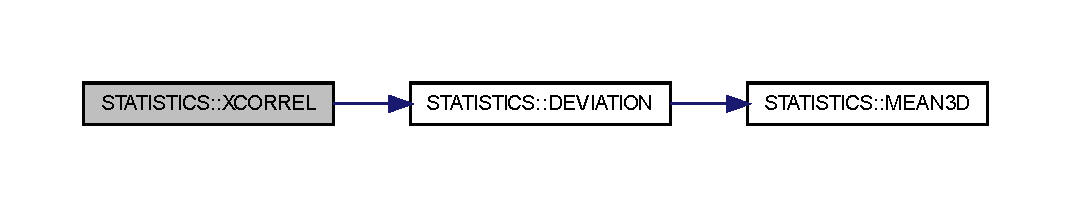
\includegraphics[width=400pt]{namespaceSTATISTICS_a2529efc59bb06c5f2280df7277bf5c7d_cgraph}
\end{center}
\end{figure}



\hypertarget{namespaceTIMER__CLASS}{
\section{TIMER\_\-CLASS Module Reference}
\label{namespaceTIMER__CLASS}\index{TIMER\_\-CLASS@{TIMER\_\-CLASS}}
}
\subsection*{Data Types}
\begin{DoxyCompactItemize}
\item 
type \hyperlink{typeTIMER__CLASS_1_1TIMER}{TIMER}
\end{DoxyCompactItemize}
\subsection*{Variables}
\begin{DoxyCompactItemize}
\item 
INTEGER, parameter \hyperlink{namespaceTIMER__CLASS_aad0658ec4217d15cb973a454db271c59}{DBL} = SELECTED\_\-REAL\_\-KIND(p=DP)
\end{DoxyCompactItemize}


\subsection{Variable Documentation}
\hypertarget{namespaceTIMER__CLASS_aad0658ec4217d15cb973a454db271c59}{
\index{TIMER\_\-CLASS@{TIMER\_\-CLASS}!DBL@{DBL}}
\index{DBL@{DBL}!TIMER_CLASS@{TIMER\_\-CLASS}}
\subsubsection[{DBL}]{\setlength{\rightskip}{0pt plus 5cm}INTEGER,parameter {\bf TIMER\_\-CLASS::DBL} = SELECTED\_\-REAL\_\-KIND(p=DP)}}
\label{namespaceTIMER__CLASS_aad0658ec4217d15cb973a454db271c59}


Definition at line 5 of file TIMER.f90.


\chapter{Data Type Documentation}
\hypertarget{interfacePREMIXED__CLASS_1_1COMP__PROGRESS}{
\section{PREMIXED\_\-CLASS::COMP\_\-PROGRESS Interface Reference}
\label{interfacePREMIXED__CLASS_1_1COMP__PROGRESS}\index{PREMIXED\_\-CLASS::COMP\_\-PROGRESS@{PREMIXED\_\-CLASS::COMP\_\-PROGRESS}}
}
\subsection*{Public Member Functions}
\begin{DoxyCompactItemize}
\item 
subroutine \hyperlink{interfacePREMIXED__CLASS_1_1COMP__PROGRESS_aae27cb4b34d99de406053d773f83fe1e}{COMP\_\-PROGRESS} (TEMPER, PROG\_\-VAR, SPEC, SPECUB, SPECB, SAVEVAR)
\end{DoxyCompactItemize}


\subsection{Detailed Description}


Definition at line 3 of file PREMIXED.f90.



\subsection{Constructor \& Destructor Documentation}
\hypertarget{interfacePREMIXED__CLASS_1_1COMP__PROGRESS_aae27cb4b34d99de406053d773f83fe1e}{
\index{PREMIXED\_\-CLASS::COMP\_\-PROGRESS@{PREMIXED\_\-CLASS::COMP\_\-PROGRESS}!COMP\_\-PROGRESS@{COMP\_\-PROGRESS}}
\index{COMP\_\-PROGRESS@{COMP\_\-PROGRESS}!PREMIXED_CLASS::COMP_PROGRESS@{PREMIXED\_\-CLASS::COMP\_\-PROGRESS}}
\subsubsection[{COMP\_\-PROGRESS}]{\setlength{\rightskip}{0pt plus 5cm}subroutine PREMIXED\_\-CLASS::COMP\_\-PROGRESS::COMP\_\-PROGRESS (
\begin{DoxyParamCaption}
\item[{REAL(DP),dimension(:,:,:),intent(in)}]{TEMPER, }
\item[{REAL(DP),dimension(:,:,:),intent(inout)}]{PROG\_\-VAR, }
\item[{REAL(DP),dimension(:,:,:),intent(in),optional}]{SPEC, }
\item[{REAL(DP),intent(in),optional}]{SPECUB, }
\item[{REAL(DP),intent(in),optional}]{SPECB, }
\item[{LOGICAL,intent(in),optional}]{SAVEVAR}
\end{DoxyParamCaption}
)}}
\label{interfacePREMIXED__CLASS_1_1COMP__PROGRESS_aae27cb4b34d99de406053d773f83fe1e}


Definition at line 7 of file PREMIXED.f90.



The documentation for this interface was generated from the following file:\begin{DoxyCompactItemize}
\item 
/home/fdietzsc/fortran/POSTPROC/SOURCES/\hyperlink{PREMIXED_8f90}{PREMIXED.f90}\end{DoxyCompactItemize}

\hypertarget{interfaceSTATISTICS_1_1CORREL}{
\section{STATISTICS::CORREL Interface Reference}
\label{interfaceSTATISTICS_1_1CORREL}\index{STATISTICS::CORREL@{STATISTICS::CORREL}}
}
\subsection*{Public Member Functions}
\begin{DoxyCompactItemize}
\item 
subroutine \hyperlink{interfaceSTATISTICS_1_1CORREL_a206eb4c97224194622bc1108e5a541fa}{CORREL3D} (IN, NX, NY, NZ, OUT)
\begin{DoxyCompactList}\small\item\em Computes the auto-\/correlation coefficients of the 3D input array. The general definition of the auto-\/correlation (often exressed as the covariance) function is \[\mathrm{cov}(f,f)=\left(f\star f\right)(r)=\int_0^{\infty}f(x)\,f(x+r)\,dx \] One important feature of the correlation function is that is satisfies \[\mathcal{F}\{f\star f\}=(\mathcal{F}\{f\})^*\cdot\mathcal{F}\{f\}. \] In the code this allows for fast computations of the correlation function using the FFT approach. In order to get the correlation coefficients, the previously mentioned function has to be devided by standard deviations of the input arrays. \[r=\frac{\mathrm{cov}(f,f)}{\sigma_f\,\sigma_f} \] \end{DoxyCompactList}\item 
subroutine \hyperlink{interfaceSTATISTICS_1_1CORREL_aebc01ee1d1300e0d47d6984308594343}{XCORREL} (IN1, IN2, NX, NY, NZ, OUT)
\begin{DoxyCompactList}\small\item\em Computes the cross-\/correlation coefficients of the 3D input arrays. The general definition of the cross-\/correlation (often exressed as the covariance) function is \[\mathrm{cov}(f,g)=\left(f\star g\right)(r)=\int_0^{\infty}f(x)\,g(x+r)\,dx \] One important feature of the correlation function is that is satisfies \[\mathcal{F}\{f\star g\}=(\mathcal{F}\{f\})^*\cdot\mathcal{F}\{g\}. \] In the code this allows for fast computations of the correlation function using the FFT approach. In order to get the correlation coefficients, the previously mentioned function has to be devided by standard deviations of the input arrays. \[r=\frac{\mathrm{cov}(f,g)}{\sigma_f\,\sigma_g} \] Computes the cross-\/correlation of the 3D input array \end{DoxyCompactList}\end{DoxyCompactItemize}


\subsection{Detailed Description}


Definition at line 18 of file STATISTICS.f90.



\subsection{Member Function/Subroutine Documentation}
\hypertarget{interfaceSTATISTICS_1_1CORREL_a206eb4c97224194622bc1108e5a541fa}{
\index{STATISTICS::CORREL@{STATISTICS::CORREL}!CORREL3D@{CORREL3D}}
\index{CORREL3D@{CORREL3D}!STATISTICS::CORREL@{STATISTICS::CORREL}}
\subsubsection[{CORREL3D}]{\setlength{\rightskip}{0pt plus 5cm}subroutine STATISTICS::CORREL::CORREL3D (
\begin{DoxyParamCaption}
\item[{COMPLEX(DPC),dimension(:,:,:),intent(in)}]{IN, }
\item[{INTEGER(SP)}]{NX, }
\item[{INTEGER(SP)}]{NY, }
\item[{INTEGER(SP)}]{NZ, }
\item[{COMPLEX(DPC),dimension(:,:,:),intent(inout)}]{OUT}
\end{DoxyParamCaption}
)}}
\label{interfaceSTATISTICS_1_1CORREL_a206eb4c97224194622bc1108e5a541fa}


Computes the auto-\/correlation coefficients of the 3D input array. The general definition of the auto-\/correlation (often exressed as the covariance) function is \[\mathrm{cov}(f,f)=\left(f\star f\right)(r)=\int_0^{\infty}f(x)\,f(x+r)\,dx \] One important feature of the correlation function is that is satisfies \[\mathcal{F}\{f\star f\}=(\mathcal{F}\{f\})^*\cdot\mathcal{F}\{f\}. \] In the code this allows for fast computations of the correlation function using the FFT approach. In order to get the correlation coefficients, the previously mentioned function has to be devided by standard deviations of the input arrays. \[r=\frac{\mathrm{cov}(f,f)}{\sigma_f\,\sigma_f} \] 

\begin{DoxyAuthor}{Author}
Felix Dietzsch Computes the auto-\/correlation coefficients of the 3D input array 
\end{DoxyAuthor}

\begin{DoxyParams}[1]{Parameters}
\mbox{\tt in}  & {\em IN} & 3D array for the computation of the 3D auto-\/correlation coefficients \\
\hline
\mbox{\tt in}  & {\em NX} & Number of nodes in x direction \\
\hline
\mbox{\tt in}  & {\em NY} & Number of nodes in y direction \\
\hline
\mbox{\tt in}  & {\em NZ} & Number of nodes in z direction \\
\hline
\mbox{\tt out}  & {\em OUT} & 3D array of auto-\/correlation coeffcients \\
\hline
\end{DoxyParams}


Definition at line 416 of file STATISTICS.f90.

\hypertarget{interfaceSTATISTICS_1_1CORREL_aebc01ee1d1300e0d47d6984308594343}{
\index{STATISTICS::CORREL@{STATISTICS::CORREL}!XCORREL@{XCORREL}}
\index{XCORREL@{XCORREL}!STATISTICS::CORREL@{STATISTICS::CORREL}}
\subsubsection[{XCORREL}]{\setlength{\rightskip}{0pt plus 5cm}subroutine STATISTICS::CORREL::XCORREL (
\begin{DoxyParamCaption}
\item[{COMPLEX(DPC),dimension(:,:,:),intent(in)}]{IN1, }
\item[{COMPLEX(DPC),dimension(:,:,:),intent(in)}]{IN2, }
\item[{INTEGER(SP)}]{NX, }
\item[{INTEGER(SP)}]{NY, }
\item[{INTEGER(SP)}]{NZ, }
\item[{COMPLEX(DPC),dimension(:,:,:),intent(inout)}]{OUT}
\end{DoxyParamCaption}
)}}
\label{interfaceSTATISTICS_1_1CORREL_aebc01ee1d1300e0d47d6984308594343}


Computes the cross-\/correlation coefficients of the 3D input arrays. The general definition of the cross-\/correlation (often exressed as the covariance) function is \[\mathrm{cov}(f,g)=\left(f\star g\right)(r)=\int_0^{\infty}f(x)\,g(x+r)\,dx \] One important feature of the correlation function is that is satisfies \[\mathcal{F}\{f\star g\}=(\mathcal{F}\{f\})^*\cdot\mathcal{F}\{g\}. \] In the code this allows for fast computations of the correlation function using the FFT approach. In order to get the correlation coefficients, the previously mentioned function has to be devided by standard deviations of the input arrays. \[r=\frac{\mathrm{cov}(f,g)}{\sigma_f\,\sigma_g} \] Computes the cross-\/correlation of the 3D input array 

\begin{DoxyAuthor}{Author}
Felix Dietzsch 
\end{DoxyAuthor}

\begin{DoxyParams}[1]{Parameters}
\mbox{\tt in}  & {\em IN1} & 3D array for the computation of the 3D cross-\/correlation coefficients \\
\hline
\mbox{\tt in}  & {\em IN2} & 3D array for the computation of the 3D cross-\/correlation coefficients \\
\hline
\mbox{\tt in}  & {\em NX} & Number of nodes in x direction \\
\hline
\mbox{\tt in}  & {\em NY} & Number of nodes in y direction \\
\hline
\mbox{\tt in}  & {\em NZ} & Number of nodes in z direction \\
\hline
\mbox{\tt out}  & {\em OUT} & 3D array of cross-\/correlation coeffcients \\
\hline
\end{DoxyParams}


Definition at line 485 of file STATISTICS.f90.



The documentation for this interface was generated from the following file:\begin{DoxyCompactItemize}
\item 
/home/fdietzsc/fortran/POSTPROC/SOURCES/\hyperlink{STATISTICS_8f90}{STATISTICS.f90}\end{DoxyCompactItemize}

\hypertarget{interfaceSTATISTICS_1_1DEVIAT}{
\section{STATISTICS::DEVIAT Interface Reference}
\label{interfaceSTATISTICS_1_1DEVIAT}\index{STATISTICS::DEVIAT@{STATISTICS::DEVIAT}}
}
\subsection*{Public Member Functions}
\begin{DoxyCompactItemize}
\item 
subroutine \hyperlink{interfaceSTATISTICS_1_1DEVIAT_a8a730e84fa8632aae538e98a69718d8d}{DEVIATION} (VELO, NX, NY, NZ, SIGMA)
\begin{DoxyCompactList}\small\item\em Computes the standard deviation of the 3D input array. It is computed according to \[\sigma = \sqrt{\frac{1}{N} \sum_{i=1}^N (x_i - \mu)^2}, {\rm \ \ where\ \ } \mu = \frac{1}{N} \sum_{i=1}^N x_i. \] \end{DoxyCompactList}\end{DoxyCompactItemize}


\subsection{Detailed Description}


Definition at line 27 of file STATISTICS.f90.



\subsection{Member Function/Subroutine Documentation}
\hypertarget{interfaceSTATISTICS_1_1DEVIAT_a8a730e84fa8632aae538e98a69718d8d}{
\index{STATISTICS::DEVIAT@{STATISTICS::DEVIAT}!DEVIATION@{DEVIATION}}
\index{DEVIATION@{DEVIATION}!STATISTICS::DEVIAT@{STATISTICS::DEVIAT}}
\subsubsection[{DEVIATION}]{\setlength{\rightskip}{0pt plus 5cm}subroutine STATISTICS::DEVIAT::DEVIATION (
\begin{DoxyParamCaption}
\item[{REAL(DP),dimension(:,:,:)}]{VELO, }
\item[{INTEGER(SP)}]{NX, }
\item[{INTEGER(SP)}]{NY, }
\item[{}]{NZ, }
\item[{REAL(DP)}]{SIGMA}
\end{DoxyParamCaption}
)}}
\label{interfaceSTATISTICS_1_1DEVIAT_a8a730e84fa8632aae538e98a69718d8d}


Computes the standard deviation of the 3D input array. It is computed according to \[\sigma = \sqrt{\frac{1}{N} \sum_{i=1}^N (x_i - \mu)^2}, {\rm \ \ where\ \ } \mu = \frac{1}{N} \sum_{i=1}^N x_i. \] 

\begin{DoxyAuthor}{Author}
Felix Dietzsch Computes the standard deviation of the 3D input array. 
\end{DoxyAuthor}

\begin{DoxyParams}[1]{Parameters}
\mbox{\tt in}  & {\em VELO} & 3D array of which the deviation is to be computed \\
\hline
\mbox{\tt in}  & {\em NX} & Number of nodes in x direction \\
\hline
\mbox{\tt in}  & {\em NY} & Number of nodes in y direction \\
\hline
\mbox{\tt in}  & {\em NZ} & Number of nodes in z direction \\
\hline
\mbox{\tt out}  & {\em SIGMA} & Standard deviation of the input array velocities \\
\hline
\end{DoxyParams}


Definition at line 319 of file STATISTICS.f90.



The documentation for this interface was generated from the following file:\begin{DoxyCompactItemize}
\item 
/home/fdietzsc/fortran/POSTPROC/SOURCES/\hyperlink{STATISTICS_8f90}{STATISTICS.f90}\end{DoxyCompactItemize}

\hypertarget{typeFIELD__CLASS_1_1field}{
\section{FIELD\_\-CLASS::field Type Reference}
\label{typeFIELD__CLASS_1_1field}\index{FIELD\_\-CLASS::field@{FIELD\_\-CLASS::field}}
}
\subsection*{Public Member Functions}
\begin{DoxyCompactItemize}
\item 
PROCEDURE, public \hyperlink{typeFIELD__CLASS_1_1field_a8e023a1758937c8f025b8b39bb0a2610}{create\_\-2d} =$>$ alloc\_\-array2d\_\-f
\item 
PROCEDURE, public \hyperlink{typeFIELD__CLASS_1_1field_adf2bc2dbcc092c8ba80c752fc708746b}{create\_\-3d} =$>$ alloc\_\-array3d\_\-f
\end{DoxyCompactItemize}
\subsection*{Public Attributes}
\begin{DoxyCompactItemize}
\item 
INTEGER(SP) \hyperlink{typeFIELD__CLASS_1_1field_a370710dc9047b03120f6c7a17403805d}{dim1}
\item 
INTEGER(SP) \hyperlink{typeFIELD__CLASS_1_1field_a44feaba31e860b83d47d9a3daee820e4}{dim2}
\item 
INTEGER(SP) \hyperlink{typeFIELD__CLASS_1_1field_a53ff81eafe27728c0e0e3ace291e767f}{dim3}
\item 
REAL(DP), dimension(:,:,:), allocatable \hyperlink{typeFIELD__CLASS_1_1field_aff70dcbe5b209245d1ea9cb44c55a8b1}{array}
\item 
INTEGER(SP) \hyperlink{typeFIELD__CLASS_1_1field_abcd9a96e4cd329576b3dca7ff0ccfa0a}{ierr}
\end{DoxyCompactItemize}


\subsection{Detailed Description}


Definition at line 4 of file ALGEBRA.f90.



\subsection{Member Function/Subroutine Documentation}
\hypertarget{typeFIELD__CLASS_1_1field_a8e023a1758937c8f025b8b39bb0a2610}{
\index{FIELD\_\-CLASS::field@{FIELD\_\-CLASS::field}!create\_\-2d@{create\_\-2d}}
\index{create\_\-2d@{create\_\-2d}!FIELD_CLASS::field@{FIELD\_\-CLASS::field}}
\subsubsection[{create\_\-2d}]{\setlength{\rightskip}{0pt plus 5cm}PROCEDURE,public FIELD\_\-CLASS::field::create\_\-2d (
\begin{DoxyParamCaption}
{}
\end{DoxyParamCaption}
)}}
\label{typeFIELD__CLASS_1_1field_a8e023a1758937c8f025b8b39bb0a2610}


Definition at line 12 of file ALGEBRA.f90.

\hypertarget{typeFIELD__CLASS_1_1field_adf2bc2dbcc092c8ba80c752fc708746b}{
\index{FIELD\_\-CLASS::field@{FIELD\_\-CLASS::field}!create\_\-3d@{create\_\-3d}}
\index{create\_\-3d@{create\_\-3d}!FIELD_CLASS::field@{FIELD\_\-CLASS::field}}
\subsubsection[{create\_\-3d}]{\setlength{\rightskip}{0pt plus 5cm}PROCEDURE,public FIELD\_\-CLASS::field::create\_\-3d (
\begin{DoxyParamCaption}
{}
\end{DoxyParamCaption}
)}}
\label{typeFIELD__CLASS_1_1field_adf2bc2dbcc092c8ba80c752fc708746b}


Definition at line 13 of file ALGEBRA.f90.



\subsection{Member Data Documentation}
\hypertarget{typeFIELD__CLASS_1_1field_aff70dcbe5b209245d1ea9cb44c55a8b1}{
\index{FIELD\_\-CLASS::field@{FIELD\_\-CLASS::field}!array@{array}}
\index{array@{array}!FIELD_CLASS::field@{FIELD\_\-CLASS::field}}
\subsubsection[{array}]{\setlength{\rightskip}{0pt plus 5cm}REAL(DP),dimension(:,:,:),allocatable {\bf FIELD\_\-CLASS::field::array}}}
\label{typeFIELD__CLASS_1_1field_aff70dcbe5b209245d1ea9cb44c55a8b1}


Definition at line 9 of file ALGEBRA.f90.

\hypertarget{typeFIELD__CLASS_1_1field_a370710dc9047b03120f6c7a17403805d}{
\index{FIELD\_\-CLASS::field@{FIELD\_\-CLASS::field}!dim1@{dim1}}
\index{dim1@{dim1}!FIELD_CLASS::field@{FIELD\_\-CLASS::field}}
\subsubsection[{dim1}]{\setlength{\rightskip}{0pt plus 5cm}INTEGER(SP) {\bf FIELD\_\-CLASS::field::dim1}}}
\label{typeFIELD__CLASS_1_1field_a370710dc9047b03120f6c7a17403805d}


Definition at line 6 of file ALGEBRA.f90.

\hypertarget{typeFIELD__CLASS_1_1field_a44feaba31e860b83d47d9a3daee820e4}{
\index{FIELD\_\-CLASS::field@{FIELD\_\-CLASS::field}!dim2@{dim2}}
\index{dim2@{dim2}!FIELD_CLASS::field@{FIELD\_\-CLASS::field}}
\subsubsection[{dim2}]{\setlength{\rightskip}{0pt plus 5cm}INTEGER(SP) {\bf FIELD\_\-CLASS::field::dim2}}}
\label{typeFIELD__CLASS_1_1field_a44feaba31e860b83d47d9a3daee820e4}


Definition at line 7 of file ALGEBRA.f90.

\hypertarget{typeFIELD__CLASS_1_1field_a53ff81eafe27728c0e0e3ace291e767f}{
\index{FIELD\_\-CLASS::field@{FIELD\_\-CLASS::field}!dim3@{dim3}}
\index{dim3@{dim3}!FIELD_CLASS::field@{FIELD\_\-CLASS::field}}
\subsubsection[{dim3}]{\setlength{\rightskip}{0pt plus 5cm}INTEGER(SP) {\bf FIELD\_\-CLASS::field::dim3}}}
\label{typeFIELD__CLASS_1_1field_a53ff81eafe27728c0e0e3ace291e767f}


Definition at line 8 of file ALGEBRA.f90.

\hypertarget{typeFIELD__CLASS_1_1field_abcd9a96e4cd329576b3dca7ff0ccfa0a}{
\index{FIELD\_\-CLASS::field@{FIELD\_\-CLASS::field}!ierr@{ierr}}
\index{ierr@{ierr}!FIELD_CLASS::field@{FIELD\_\-CLASS::field}}
\subsubsection[{ierr}]{\setlength{\rightskip}{0pt plus 5cm}INTEGER(SP) {\bf FIELD\_\-CLASS::field::ierr}}}
\label{typeFIELD__CLASS_1_1field_abcd9a96e4cd329576b3dca7ff0ccfa0a}


Definition at line 10 of file ALGEBRA.f90.



The documentation for this type was generated from the following file:\begin{DoxyCompactItemize}
\item 
/home/fdietzsc/fortran/POSTPROC/SOURCES/\hyperlink{ALGEBRA_8f90}{ALGEBRA.f90}\end{DoxyCompactItemize}

\hypertarget{interfaceIO__CLASS_1_1INDEXING}{
\section{IO\_\-CLASS::INDEXING Interface Reference}
\label{interfaceIO__CLASS_1_1INDEXING}\index{IO\_\-CLASS::INDEXING@{IO\_\-CLASS::INDEXING}}
}
\subsection*{Public Member Functions}
\begin{DoxyCompactItemize}
\item 
subroutine \hyperlink{interfaceIO__CLASS_1_1INDEXING_acb48f867c8c92f5fb1d01493d8e53f99}{INDEXING} (COORD, NUMBER\_\-OF\_\-NODES, INDX, NX, INDY, NY, INDZ, NZ)
\end{DoxyCompactItemize}


\subsection{Detailed Description}


Definition at line 16 of file IO.f90.



\subsection{Constructor \& Destructor Documentation}
\hypertarget{interfaceIO__CLASS_1_1INDEXING_acb48f867c8c92f5fb1d01493d8e53f99}{
\index{IO\_\-CLASS::INDEXING@{IO\_\-CLASS::INDEXING}!INDEXING@{INDEXING}}
\index{INDEXING@{INDEXING}!IO_CLASS::INDEXING@{IO\_\-CLASS::INDEXING}}
\subsubsection[{INDEXING}]{\setlength{\rightskip}{0pt plus 5cm}subroutine IO\_\-CLASS::INDEXING::INDEXING (
\begin{DoxyParamCaption}
\item[{REAL(DP),dimension(:,:)}]{COORD, }
\item[{INTEGER(SP)}]{NUMBER\_\-OF\_\-NODES, }
\item[{INTEGER(SP),dimension(:),intent(inout)}]{INDX, }
\item[{INTEGER(SP),intent(inout)}]{NX, }
\item[{INTEGER(SP),dimension(:),intent(inout)}]{INDY, }
\item[{INTEGER(SP),intent(inout)}]{NY, }
\item[{INTEGER(SP),dimension(:),intent(inout),optional}]{INDZ, }
\item[{INTEGER(SP),intent(inout),optional}]{NZ}
\end{DoxyParamCaption}
)}}
\label{interfaceIO__CLASS_1_1INDEXING_acb48f867c8c92f5fb1d01493d8e53f99}


Definition at line 17 of file IO.f90.



The documentation for this interface was generated from the following file:\begin{DoxyCompactItemize}
\item 
/home/fdietzsc/fortran/POSTPROC/SOURCES/\hyperlink{IO_8f90}{IO.f90}\end{DoxyCompactItemize}

\hypertarget{typeIO__CLASS_1_1IO}{
\section{IO\_\-CLASS::IO Type Reference}
\label{typeIO__CLASS_1_1IO}\index{IO\_\-CLASS::IO@{IO\_\-CLASS::IO}}
}
\subsection*{Public Member Functions}
\begin{DoxyCompactItemize}
\item 
PROCEDURE, public \hyperlink{typeIO__CLASS_1_1IO_a4e7f9793856d178a294424a41956b06d}{file\_\-stats} =$>$ read\_\-file\_\-sub
\item 
PROCEDURE, public \hyperlink{typeIO__CLASS_1_1IO_a2a95f54a70215c2a7f4404998959e254}{NOL} =$>$ number\_\-of\_\-lines\_\-f
\item 
PROCEDURE, public \hyperlink{typeIO__CLASS_1_1IO_aa5e54a8b52ad93ea8db77b0aec13e628}{NON} =$>$ number\_\-of\_\-nodes\_\-f
\item 
PROCEDURE, public \hyperlink{typeIO__CLASS_1_1IO_ad813b656a5fa827ba84f34bd8f9b87bb}{NX} =$>$ number\_\-of\_\-nodes\_\-x\_\-f
\item 
PROCEDURE, public \hyperlink{typeIO__CLASS_1_1IO_aadc595d12b6ccecae3347240c9da9436}{NY} =$>$ number\_\-of\_\-nodes\_\-y\_\-f
\item 
PROCEDURE, public \hyperlink{typeIO__CLASS_1_1IO_ae711f2f0d918f3f40eacd0cd74ab29e4}{NZ} =$>$ number\_\-of\_\-nodes\_\-z\_\-f
\item 
PROCEDURE, public \hyperlink{typeIO__CLASS_1_1IO_ab7f25108ce89b8b8a037698b04449214}{read\_\-file} =$>$ read\_\-dummy\_\-sub
\item 
PROCEDURE, public \hyperlink{typeIO__CLASS_1_1IO_a31154428dde5e51b86a591977acab9f4}{field} =$>$ field\_\-f
\end{DoxyCompactItemize}
\subsection*{Public Attributes}
\begin{DoxyCompactItemize}
\item 
INTEGER(SP) \hyperlink{typeIO__CLASS_1_1IO_a3b70c5d8c06d577a282d4987fbdcfa5e}{NOLINES}
\item 
INTEGER(SP) \hyperlink{typeIO__CLASS_1_1IO_afb096dbfeea6075e4867273b2d2cd282}{NONODES}
\item 
INTEGER(SP) \hyperlink{typeIO__CLASS_1_1IO_a3fe805b71504c0d8d043bb0bc22b9ec1}{NONX}
\item 
INTEGER(SP) \hyperlink{typeIO__CLASS_1_1IO_a1259b785f9bba0ff1f11191b9f8a3b8d}{NONY}
\item 
INTEGER(SP) \hyperlink{typeIO__CLASS_1_1IO_ad396a56353638ec204e9fff5ae71202c}{NONZ}
\item 
INTEGER(SP) \hyperlink{typeIO__CLASS_1_1IO_ae4de46da7a025c4f4f8e8d6241418ee9}{DIM}
\item 
REAL(DP), dimension(:,:), pointer \hyperlink{typeIO__CLASS_1_1IO_a28657cb15afcf0b2725d64be12ab7c01}{dummy}
\end{DoxyCompactItemize}


\subsection{Detailed Description}


Definition at line 142 of file IO.f90.



\subsection{Member Function/Subroutine Documentation}
\hypertarget{typeIO__CLASS_1_1IO_a31154428dde5e51b86a591977acab9f4}{
\index{IO\_\-CLASS::IO@{IO\_\-CLASS::IO}!field@{field}}
\index{field@{field}!IO_CLASS::IO@{IO\_\-CLASS::IO}}
\subsubsection[{field}]{\setlength{\rightskip}{0pt plus 5cm}PROCEDURE,public IO\_\-CLASS::IO::field (
\begin{DoxyParamCaption}
{}
\end{DoxyParamCaption}
)}}
\label{typeIO__CLASS_1_1IO_a31154428dde5e51b86a591977acab9f4}


Definition at line 159 of file IO.f90.



References IO\_\-CLASS::field\_\-f().



Here is the call graph for this function:
\nopagebreak
\begin{figure}[H]
\begin{center}
\leavevmode
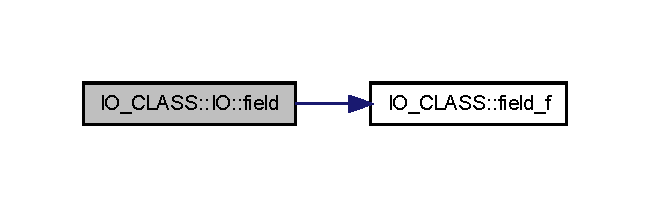
\includegraphics[width=312pt]{typeIO__CLASS_1_1IO_a31154428dde5e51b86a591977acab9f4_cgraph}
\end{center}
\end{figure}


\hypertarget{typeIO__CLASS_1_1IO_a4e7f9793856d178a294424a41956b06d}{
\index{IO\_\-CLASS::IO@{IO\_\-CLASS::IO}!file\_\-stats@{file\_\-stats}}
\index{file\_\-stats@{file\_\-stats}!IO_CLASS::IO@{IO\_\-CLASS::IO}}
\subsubsection[{file\_\-stats}]{\setlength{\rightskip}{0pt plus 5cm}PROCEDURE,public IO\_\-CLASS::IO::file\_\-stats (
\begin{DoxyParamCaption}
{}
\end{DoxyParamCaption}
)}}
\label{typeIO__CLASS_1_1IO_a4e7f9793856d178a294424a41956b06d}


Definition at line 152 of file IO.f90.

\hypertarget{typeIO__CLASS_1_1IO_a2a95f54a70215c2a7f4404998959e254}{
\index{IO\_\-CLASS::IO@{IO\_\-CLASS::IO}!NOL@{NOL}}
\index{NOL@{NOL}!IO_CLASS::IO@{IO\_\-CLASS::IO}}
\subsubsection[{NOL}]{\setlength{\rightskip}{0pt plus 5cm}PROCEDURE,public IO\_\-CLASS::IO::NOL (
\begin{DoxyParamCaption}
{}
\end{DoxyParamCaption}
)}}
\label{typeIO__CLASS_1_1IO_a2a95f54a70215c2a7f4404998959e254}


Definition at line 153 of file IO.f90.

\hypertarget{typeIO__CLASS_1_1IO_aa5e54a8b52ad93ea8db77b0aec13e628}{
\index{IO\_\-CLASS::IO@{IO\_\-CLASS::IO}!NON@{NON}}
\index{NON@{NON}!IO_CLASS::IO@{IO\_\-CLASS::IO}}
\subsubsection[{NON}]{\setlength{\rightskip}{0pt plus 5cm}PROCEDURE,public IO\_\-CLASS::IO::NON (
\begin{DoxyParamCaption}
{}
\end{DoxyParamCaption}
)}}
\label{typeIO__CLASS_1_1IO_aa5e54a8b52ad93ea8db77b0aec13e628}


Definition at line 154 of file IO.f90.

\hypertarget{typeIO__CLASS_1_1IO_ad813b656a5fa827ba84f34bd8f9b87bb}{
\index{IO\_\-CLASS::IO@{IO\_\-CLASS::IO}!NX@{NX}}
\index{NX@{NX}!IO_CLASS::IO@{IO\_\-CLASS::IO}}
\subsubsection[{NX}]{\setlength{\rightskip}{0pt plus 5cm}PROCEDURE,public IO\_\-CLASS::IO::NX (
\begin{DoxyParamCaption}
{}
\end{DoxyParamCaption}
)}}
\label{typeIO__CLASS_1_1IO_ad813b656a5fa827ba84f34bd8f9b87bb}


Definition at line 155 of file IO.f90.



References IO\_\-CLASS::number\_\-of\_\-nodes\_\-x\_\-f().



Here is the call graph for this function:
\nopagebreak
\begin{figure}[H]
\begin{center}
\leavevmode
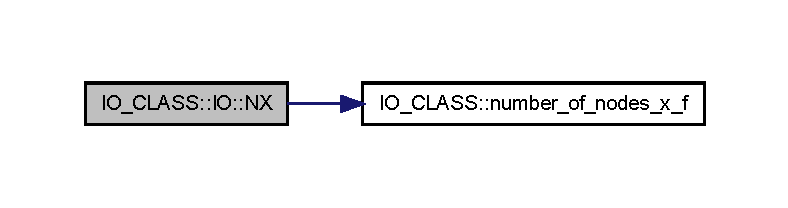
\includegraphics[width=378pt]{typeIO__CLASS_1_1IO_ad813b656a5fa827ba84f34bd8f9b87bb_cgraph}
\end{center}
\end{figure}


\hypertarget{typeIO__CLASS_1_1IO_aadc595d12b6ccecae3347240c9da9436}{
\index{IO\_\-CLASS::IO@{IO\_\-CLASS::IO}!NY@{NY}}
\index{NY@{NY}!IO_CLASS::IO@{IO\_\-CLASS::IO}}
\subsubsection[{NY}]{\setlength{\rightskip}{0pt plus 5cm}PROCEDURE,public IO\_\-CLASS::IO::NY (
\begin{DoxyParamCaption}
{}
\end{DoxyParamCaption}
)}}
\label{typeIO__CLASS_1_1IO_aadc595d12b6ccecae3347240c9da9436}


Definition at line 156 of file IO.f90.



References IO\_\-CLASS::number\_\-of\_\-nodes\_\-y\_\-f().



Here is the call graph for this function:
\nopagebreak
\begin{figure}[H]
\begin{center}
\leavevmode
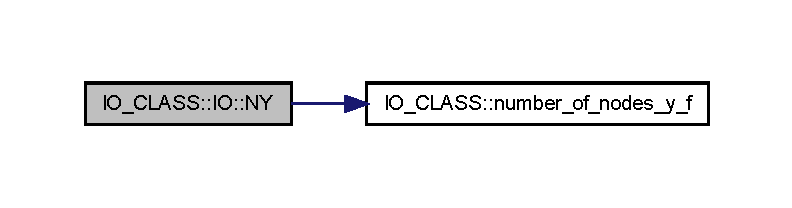
\includegraphics[width=380pt]{typeIO__CLASS_1_1IO_aadc595d12b6ccecae3347240c9da9436_cgraph}
\end{center}
\end{figure}


\hypertarget{typeIO__CLASS_1_1IO_ae711f2f0d918f3f40eacd0cd74ab29e4}{
\index{IO\_\-CLASS::IO@{IO\_\-CLASS::IO}!NZ@{NZ}}
\index{NZ@{NZ}!IO_CLASS::IO@{IO\_\-CLASS::IO}}
\subsubsection[{NZ}]{\setlength{\rightskip}{0pt plus 5cm}PROCEDURE,public IO\_\-CLASS::IO::NZ (
\begin{DoxyParamCaption}
{}
\end{DoxyParamCaption}
)}}
\label{typeIO__CLASS_1_1IO_ae711f2f0d918f3f40eacd0cd74ab29e4}


Definition at line 157 of file IO.f90.



References IO\_\-CLASS::number\_\-of\_\-nodes\_\-z\_\-f().



Here is the call graph for this function:
\nopagebreak
\begin{figure}[H]
\begin{center}
\leavevmode
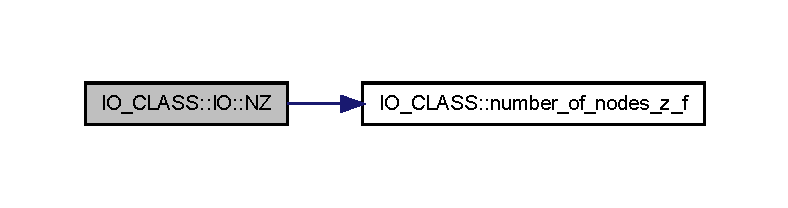
\includegraphics[width=378pt]{typeIO__CLASS_1_1IO_ae711f2f0d918f3f40eacd0cd74ab29e4_cgraph}
\end{center}
\end{figure}


\hypertarget{typeIO__CLASS_1_1IO_ab7f25108ce89b8b8a037698b04449214}{
\index{IO\_\-CLASS::IO@{IO\_\-CLASS::IO}!read\_\-file@{read\_\-file}}
\index{read\_\-file@{read\_\-file}!IO_CLASS::IO@{IO\_\-CLASS::IO}}
\subsubsection[{read\_\-file}]{\setlength{\rightskip}{0pt plus 5cm}PROCEDURE,public IO\_\-CLASS::IO::read\_\-file (
\begin{DoxyParamCaption}
{}
\end{DoxyParamCaption}
)}}
\label{typeIO__CLASS_1_1IO_ab7f25108ce89b8b8a037698b04449214}


Definition at line 158 of file IO.f90.



References IO\_\-CLASS::read\_\-dummy\_\-sub().



Here is the call graph for this function:
\nopagebreak
\begin{figure}[H]
\begin{center}
\leavevmode
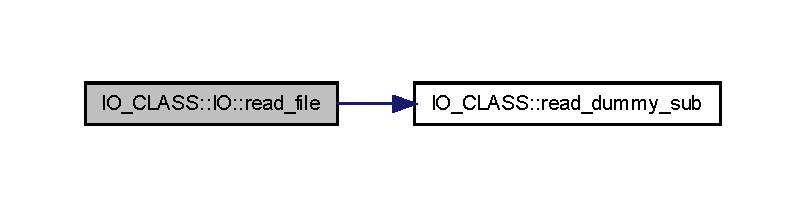
\includegraphics[width=386pt]{typeIO__CLASS_1_1IO_ab7f25108ce89b8b8a037698b04449214_cgraph}
\end{center}
\end{figure}




\subsection{Member Data Documentation}
\hypertarget{typeIO__CLASS_1_1IO_ae4de46da7a025c4f4f8e8d6241418ee9}{
\index{IO\_\-CLASS::IO@{IO\_\-CLASS::IO}!DIM@{DIM}}
\index{DIM@{DIM}!IO_CLASS::IO@{IO\_\-CLASS::IO}}
\subsubsection[{DIM}]{\setlength{\rightskip}{0pt plus 5cm}INTEGER(SP) {\bf IO\_\-CLASS::IO::DIM}}}
\label{typeIO__CLASS_1_1IO_ae4de46da7a025c4f4f8e8d6241418ee9}


Definition at line 149 of file IO.f90.

\hypertarget{typeIO__CLASS_1_1IO_a28657cb15afcf0b2725d64be12ab7c01}{
\index{IO\_\-CLASS::IO@{IO\_\-CLASS::IO}!dummy@{dummy}}
\index{dummy@{dummy}!IO_CLASS::IO@{IO\_\-CLASS::IO}}
\subsubsection[{dummy}]{\setlength{\rightskip}{0pt plus 5cm}REAL(DP),dimension(:,:),pointer {\bf IO\_\-CLASS::IO::dummy}}}
\label{typeIO__CLASS_1_1IO_a28657cb15afcf0b2725d64be12ab7c01}


Definition at line 150 of file IO.f90.

\hypertarget{typeIO__CLASS_1_1IO_a3b70c5d8c06d577a282d4987fbdcfa5e}{
\index{IO\_\-CLASS::IO@{IO\_\-CLASS::IO}!NOLINES@{NOLINES}}
\index{NOLINES@{NOLINES}!IO_CLASS::IO@{IO\_\-CLASS::IO}}
\subsubsection[{NOLINES}]{\setlength{\rightskip}{0pt plus 5cm}INTEGER(SP) {\bf IO\_\-CLASS::IO::NOLINES}}}
\label{typeIO__CLASS_1_1IO_a3b70c5d8c06d577a282d4987fbdcfa5e}


Definition at line 144 of file IO.f90.

\hypertarget{typeIO__CLASS_1_1IO_afb096dbfeea6075e4867273b2d2cd282}{
\index{IO\_\-CLASS::IO@{IO\_\-CLASS::IO}!NONODES@{NONODES}}
\index{NONODES@{NONODES}!IO_CLASS::IO@{IO\_\-CLASS::IO}}
\subsubsection[{NONODES}]{\setlength{\rightskip}{0pt plus 5cm}INTEGER(SP) {\bf IO\_\-CLASS::IO::NONODES}}}
\label{typeIO__CLASS_1_1IO_afb096dbfeea6075e4867273b2d2cd282}


Definition at line 145 of file IO.f90.

\hypertarget{typeIO__CLASS_1_1IO_a3fe805b71504c0d8d043bb0bc22b9ec1}{
\index{IO\_\-CLASS::IO@{IO\_\-CLASS::IO}!NONX@{NONX}}
\index{NONX@{NONX}!IO_CLASS::IO@{IO\_\-CLASS::IO}}
\subsubsection[{NONX}]{\setlength{\rightskip}{0pt plus 5cm}INTEGER(SP) {\bf IO\_\-CLASS::IO::NONX}}}
\label{typeIO__CLASS_1_1IO_a3fe805b71504c0d8d043bb0bc22b9ec1}


Definition at line 146 of file IO.f90.

\hypertarget{typeIO__CLASS_1_1IO_a1259b785f9bba0ff1f11191b9f8a3b8d}{
\index{IO\_\-CLASS::IO@{IO\_\-CLASS::IO}!NONY@{NONY}}
\index{NONY@{NONY}!IO_CLASS::IO@{IO\_\-CLASS::IO}}
\subsubsection[{NONY}]{\setlength{\rightskip}{0pt plus 5cm}INTEGER(SP) {\bf IO\_\-CLASS::IO::NONY}}}
\label{typeIO__CLASS_1_1IO_a1259b785f9bba0ff1f11191b9f8a3b8d}


Definition at line 147 of file IO.f90.

\hypertarget{typeIO__CLASS_1_1IO_ad396a56353638ec204e9fff5ae71202c}{
\index{IO\_\-CLASS::IO@{IO\_\-CLASS::IO}!NONZ@{NONZ}}
\index{NONZ@{NONZ}!IO_CLASS::IO@{IO\_\-CLASS::IO}}
\subsubsection[{NONZ}]{\setlength{\rightskip}{0pt plus 5cm}INTEGER(SP) {\bf IO\_\-CLASS::IO::NONZ}}}
\label{typeIO__CLASS_1_1IO_ad396a56353638ec204e9fff5ae71202c}


Definition at line 148 of file IO.f90.



The documentation for this type was generated from the following file:\begin{DoxyCompactItemize}
\item 
/home/fdietzsc/fortran/POSTPROC/SOURCES/\hyperlink{IO_8f90}{IO.f90}\end{DoxyCompactItemize}

\hypertarget{interfaceSTATISTICS_1_1MEAN}{
\section{STATISTICS::MEAN Interface Reference}
\label{interfaceSTATISTICS_1_1MEAN}\index{STATISTICS::MEAN@{STATISTICS::MEAN}}
}
\subsection*{Public Member Functions}
\begin{DoxyCompactItemize}
\item 
subroutine \hyperlink{interfaceSTATISTICS_1_1MEAN_a97da6fad38ebdadf885aad5e633df4fc}{MEAN1D} (M, NX)
\item 
subroutine \hyperlink{interfaceSTATISTICS_1_1MEAN_ad7780f2b91da10d31731a34b882a211b}{MEAN3D} (M, NX, NY, NZ, \hyperlink{interfaceSTATISTICS_1_1MEAN}{MEAN})
\begin{DoxyCompactList}\small\item\em Shifts the input array towards the zero frequencies. \end{DoxyCompactList}\item 
subroutine \hyperlink{interfaceSTATISTICS_1_1MEAN_a7211c5a2a32311a19d04ab567c005d46}{MEAN4D} (M, NX, NY, NZ, DIM, \hyperlink{interfaceSTATISTICS_1_1MEAN}{MEAN})
\end{DoxyCompactItemize}


\subsection{Detailed Description}


Definition at line 15 of file STATISTICS.f90.



\subsection{Member Function/Subroutine Documentation}
\hypertarget{interfaceSTATISTICS_1_1MEAN_a97da6fad38ebdadf885aad5e633df4fc}{
\index{STATISTICS::MEAN@{STATISTICS::MEAN}!MEAN1D@{MEAN1D}}
\index{MEAN1D@{MEAN1D}!STATISTICS::MEAN@{STATISTICS::MEAN}}
\subsubsection[{MEAN1D}]{\setlength{\rightskip}{0pt plus 5cm}subroutine STATISTICS::MEAN::MEAN1D (
\begin{DoxyParamCaption}
\item[{REAL(DP),dimension(:)}]{M, }
\item[{INTEGER(SP)}]{NX}
\end{DoxyParamCaption}
)}}
\label{interfaceSTATISTICS_1_1MEAN_a97da6fad38ebdadf885aad5e633df4fc}


Definition at line 526 of file STATISTICS.f90.

\hypertarget{interfaceSTATISTICS_1_1MEAN_ad7780f2b91da10d31731a34b882a211b}{
\index{STATISTICS::MEAN@{STATISTICS::MEAN}!MEAN3D@{MEAN3D}}
\index{MEAN3D@{MEAN3D}!STATISTICS::MEAN@{STATISTICS::MEAN}}
\subsubsection[{MEAN3D}]{\setlength{\rightskip}{0pt plus 5cm}subroutine STATISTICS::MEAN::MEAN3D (
\begin{DoxyParamCaption}
\item[{REAL(DP),dimension(:,:,:)}]{M, }
\item[{INTEGER(SP)}]{NX, }
\item[{INTEGER(SP)}]{NY, }
\item[{}]{NZ, }
\item[{REAL(DP)}]{MEAN}
\end{DoxyParamCaption}
)}}
\label{interfaceSTATISTICS_1_1MEAN_ad7780f2b91da10d31731a34b882a211b}


Shifts the input array towards the zero frequencies. 

\begin{DoxyAuthor}{Author}
Felix Dietzsch 
\end{DoxyAuthor}

\begin{DoxyParams}[1]{Parameters}
\mbox{\tt in}  & {\em M} & 3D array for the computation of the mean value \\
\hline
\mbox{\tt in}  & {\em NX} & Number of nodes in x direction \\
\hline
\mbox{\tt in}  & {\em NY} & Number of nodes in y direction \\
\hline
\mbox{\tt in}  & {\em NZ} & Number of nodes in z direction \\
\hline
\mbox{\tt out}  & {\em \hyperlink{interfaceSTATISTICS_1_1MEAN}{MEAN}} & Computed mean value \\
\hline
\end{DoxyParams}


Definition at line 547 of file STATISTICS.f90.

\hypertarget{interfaceSTATISTICS_1_1MEAN_a7211c5a2a32311a19d04ab567c005d46}{
\index{STATISTICS::MEAN@{STATISTICS::MEAN}!MEAN4D@{MEAN4D}}
\index{MEAN4D@{MEAN4D}!STATISTICS::MEAN@{STATISTICS::MEAN}}
\subsubsection[{MEAN4D}]{\setlength{\rightskip}{0pt plus 5cm}subroutine STATISTICS::MEAN::MEAN4D (
\begin{DoxyParamCaption}
\item[{REAL(DP),dimension(:,:,:,:)}]{M, }
\item[{INTEGER(SP)}]{NX, }
\item[{INTEGER(SP)}]{NY, }
\item[{}]{NZ, }
\item[{INTEGER(SP)}]{DIM, }
\item[{REAL(DP)}]{MEAN}
\end{DoxyParamCaption}
)}}
\label{interfaceSTATISTICS_1_1MEAN_a7211c5a2a32311a19d04ab567c005d46}


Definition at line 556 of file STATISTICS.f90.



The documentation for this interface was generated from the following file:\begin{DoxyCompactItemize}
\item 
/home/fdietzsc/fortran/POSTPROC/SOURCES/\hyperlink{STATISTICS_8f90}{STATISTICS.f90}\end{DoxyCompactItemize}

\hypertarget{interfaceIO__CLASS_1_1READ__DIM}{
\section{IO\_\-CLASS::READ\_\-DIM Interface Reference}
\label{interfaceIO__CLASS_1_1READ__DIM}\index{IO\_\-CLASS::READ\_\-DIM@{IO\_\-CLASS::READ\_\-DIM}}
}
\subsection*{Public Member Functions}
\begin{DoxyCompactItemize}
\item 
subroutine \hyperlink{interfaceIO__CLASS_1_1READ__DIM_a718fe5a6707c3f46c8e4094c1ee58d94}{READ\_\-DIM} (FILEX, FILEY, FILEZ, DIMEN)
\end{DoxyCompactItemize}


\subsection{Detailed Description}


Definition at line 43 of file IO.f90.



\subsection{Constructor \& Destructor Documentation}
\hypertarget{interfaceIO__CLASS_1_1READ__DIM_a718fe5a6707c3f46c8e4094c1ee58d94}{
\index{IO\_\-CLASS::READ\_\-DIM@{IO\_\-CLASS::READ\_\-DIM}!READ\_\-DIM@{READ\_\-DIM}}
\index{READ\_\-DIM@{READ\_\-DIM}!IO_CLASS::READ_DIM@{IO\_\-CLASS::READ\_\-DIM}}
\subsubsection[{READ\_\-DIM}]{\setlength{\rightskip}{0pt plus 5cm}subroutine IO\_\-CLASS::READ\_\-DIM::READ\_\-DIM (
\begin{DoxyParamCaption}
\item[{CHARACTER(LEN=$\ast$),intent(in)}]{FILEX, }
\item[{CHARACTER(LEN=$\ast$),intent(in)}]{FILEY, }
\item[{CHARACTER(LEN=$\ast$),intent(in)}]{FILEZ, }
\item[{INTEGER(SP),dimension(:),intent(inout)}]{DIMEN}
\end{DoxyParamCaption}
)}}
\label{interfaceIO__CLASS_1_1READ__DIM_a718fe5a6707c3f46c8e4094c1ee58d94}


Definition at line 44 of file IO.f90.



The documentation for this interface was generated from the following file:\begin{DoxyCompactItemize}
\item 
/home/fdietzsc/fortran/POSTPROC/SOURCES/\hyperlink{IO_8f90}{IO.f90}\end{DoxyCompactItemize}

\hypertarget{interfaceIO__CLASS_1_1READ__GRID}{
\section{IO\_\-CLASS::READ\_\-GRID Interface Reference}
\label{interfaceIO__CLASS_1_1READ__GRID}\index{IO\_\-CLASS::READ\_\-GRID@{IO\_\-CLASS::READ\_\-GRID}}
}
\subsection*{Public Member Functions}
\begin{DoxyCompactItemize}
\item 
subroutine \hyperlink{interfaceIO__CLASS_1_1READ__GRID_a65015fa768d8283003d4efb2e678508a}{READ\_\-GRID} (FILEX, FILEY, FILEZ, GRIDX, GRIDY, GRIDZ)
\end{DoxyCompactItemize}


\subsection{Detailed Description}


Definition at line 55 of file IO.f90.



\subsection{Constructor \& Destructor Documentation}
\hypertarget{interfaceIO__CLASS_1_1READ__GRID_a65015fa768d8283003d4efb2e678508a}{
\index{IO\_\-CLASS::READ\_\-GRID@{IO\_\-CLASS::READ\_\-GRID}!READ\_\-GRID@{READ\_\-GRID}}
\index{READ\_\-GRID@{READ\_\-GRID}!IO_CLASS::READ_GRID@{IO\_\-CLASS::READ\_\-GRID}}
\subsubsection[{READ\_\-GRID}]{\setlength{\rightskip}{0pt plus 5cm}subroutine IO\_\-CLASS::READ\_\-GRID::READ\_\-GRID (
\begin{DoxyParamCaption}
\item[{CHARACTER(LEN=$\ast$),intent(in)}]{FILEX, }
\item[{CHARACTER(LEN=$\ast$),intent(in)}]{FILEY, }
\item[{CHARACTER(LEN=$\ast$),intent(in)}]{FILEZ, }
\item[{REAL(DP),dimension(:),intent(inout)}]{GRIDX, }
\item[{REAL(DP),dimension(:),intent(inout)}]{GRIDY, }
\item[{REAL(DP),dimension(:),intent(inout)}]{GRIDZ}
\end{DoxyParamCaption}
)}}
\label{interfaceIO__CLASS_1_1READ__GRID_a65015fa768d8283003d4efb2e678508a}


Definition at line 56 of file IO.f90.



The documentation for this interface was generated from the following file:\begin{DoxyCompactItemize}
\item 
/home/fdietzsc/fortran/POSTPROC/SOURCES/\hyperlink{IO_8f90}{IO.f90}\end{DoxyCompactItemize}

\hypertarget{interfaceIO__CLASS_1_1READCOORD}{
\section{IO\_\-CLASS::READCOORD Interface Reference}
\label{interfaceIO__CLASS_1_1READCOORD}\index{IO\_\-CLASS::READCOORD@{IO\_\-CLASS::READCOORD}}
}
\subsection*{Public Member Functions}
\begin{DoxyCompactItemize}
\item 
subroutine \hyperlink{interfaceIO__CLASS_1_1READCOORD_af30aade0409d0370db275c9858b29b38}{READCOORD2D} (FILENAME, COORD)
\end{DoxyCompactItemize}


\subsection{Detailed Description}


Definition at line 32 of file IO.f90.



\subsection{Member Function/Subroutine Documentation}
\hypertarget{interfaceIO__CLASS_1_1READCOORD_af30aade0409d0370db275c9858b29b38}{
\index{IO\_\-CLASS::READCOORD@{IO\_\-CLASS::READCOORD}!READCOORD2D@{READCOORD2D}}
\index{READCOORD2D@{READCOORD2D}!IO_CLASS::READCOORD@{IO\_\-CLASS::READCOORD}}
\subsubsection[{READCOORD2D}]{\setlength{\rightskip}{0pt plus 5cm}subroutine IO\_\-CLASS::READCOORD::READCOORD2D (
\begin{DoxyParamCaption}
\item[{CHARACTER(LEN=$\ast$),intent(in)}]{FILENAME, }
\item[{REAL(DP),dimension(:,:),intent(inout)}]{COORD}
\end{DoxyParamCaption}
)}}
\label{interfaceIO__CLASS_1_1READCOORD_af30aade0409d0370db275c9858b29b38}


Definition at line 33 of file IO.f90.



The documentation for this interface was generated from the following file:\begin{DoxyCompactItemize}
\item 
/home/fdietzsc/fortran/POSTPROC/SOURCES/\hyperlink{IO_8f90}{IO.f90}\end{DoxyCompactItemize}

\hypertarget{interfaceIO__CLASS_1_1READVALUE}{
\section{IO\_\-CLASS::READVALUE Interface Reference}
\label{interfaceIO__CLASS_1_1READVALUE}\index{IO\_\-CLASS::READVALUE@{IO\_\-CLASS::READVALUE}}
}
\subsection*{Public Member Functions}
\begin{DoxyCompactItemize}
\item 
subroutine \hyperlink{interfaceIO__CLASS_1_1READVALUE_a9c5236f93e81a02d67d9cbed44cd6bb8}{READVALUE} (FILENAME, VAR)
\end{DoxyCompactItemize}


\subsection{Detailed Description}


Definition at line 69 of file IO.f90.



\subsection{Constructor \& Destructor Documentation}
\hypertarget{interfaceIO__CLASS_1_1READVALUE_a9c5236f93e81a02d67d9cbed44cd6bb8}{
\index{IO\_\-CLASS::READVALUE@{IO\_\-CLASS::READVALUE}!READVALUE@{READVALUE}}
\index{READVALUE@{READVALUE}!IO_CLASS::READVALUE@{IO\_\-CLASS::READVALUE}}
\subsubsection[{READVALUE}]{\setlength{\rightskip}{0pt plus 5cm}subroutine IO\_\-CLASS::READVALUE::READVALUE (
\begin{DoxyParamCaption}
\item[{CHARACTER(LEN=$\ast$),intent(in)}]{FILENAME, }
\item[{REAL(DP),dimension(:,:,:),intent(inout)}]{VAR}
\end{DoxyParamCaption}
)}}
\label{interfaceIO__CLASS_1_1READVALUE_a9c5236f93e81a02d67d9cbed44cd6bb8}


Definition at line 70 of file IO.f90.



The documentation for this interface was generated from the following file:\begin{DoxyCompactItemize}
\item 
/home/fdietzsc/fortran/POSTPROC/SOURCES/\hyperlink{IO_8f90}{IO.f90}\end{DoxyCompactItemize}

\hypertarget{interfaceIO__CLASS_1_1READVEL}{
\section{IO\_\-CLASS::READVEL Interface Reference}
\label{interfaceIO__CLASS_1_1READVEL}\index{IO\_\-CLASS::READVEL@{IO\_\-CLASS::READVEL}}
}
\subsection*{Public Member Functions}
\begin{DoxyCompactItemize}
\item 
subroutine \hyperlink{interfaceIO__CLASS_1_1READVEL_a483ee7ffc26a2193e971d402d487eb00}{READVEL} (FILENAME, UUX, UUY, UUZ)
\end{DoxyCompactItemize}


\subsection{Detailed Description}


Definition at line 96 of file IO.f90.



\subsection{Constructor \& Destructor Documentation}
\hypertarget{interfaceIO__CLASS_1_1READVEL_a483ee7ffc26a2193e971d402d487eb00}{
\index{IO\_\-CLASS::READVEL@{IO\_\-CLASS::READVEL}!READVEL@{READVEL}}
\index{READVEL@{READVEL}!IO_CLASS::READVEL@{IO\_\-CLASS::READVEL}}
\subsubsection[{READVEL}]{\setlength{\rightskip}{0pt plus 5cm}subroutine IO\_\-CLASS::READVEL::READVEL (
\begin{DoxyParamCaption}
\item[{CHARACTER(LEN=$\ast$),intent(in)}]{FILENAME, }
\item[{REAL(DP),dimension(:,:,:),intent(inout)}]{UUX, }
\item[{REAL(DP),dimension(:,:,:),intent(inout)}]{UUY, }
\item[{REAL(DP),dimension(:,:,:),intent(inout),optional}]{UUZ}
\end{DoxyParamCaption}
)}}
\label{interfaceIO__CLASS_1_1READVEL_a483ee7ffc26a2193e971d402d487eb00}


Definition at line 97 of file IO.f90.



The documentation for this interface was generated from the following file:\begin{DoxyCompactItemize}
\item 
/home/fdietzsc/fortran/POSTPROC/SOURCES/\hyperlink{IO_8f90}{IO.f90}\end{DoxyCompactItemize}

\hypertarget{interfaceIO__CLASS_1_1READVEL__BIN}{
\section{IO\_\-CLASS::READVEL\_\-BIN Interface Reference}
\label{interfaceIO__CLASS_1_1READVEL__BIN}\index{IO\_\-CLASS::READVEL\_\-BIN@{IO\_\-CLASS::READVEL\_\-BIN}}
}
\subsection*{Public Member Functions}
\begin{DoxyCompactItemize}
\item 
subroutine \hyperlink{interfaceIO__CLASS_1_1READVEL__BIN_a03cf0d72289bd07a3e85e9b979317efe}{READVEL\_\-BIN} (FILENAME, UX, VY, WZ)
\end{DoxyCompactItemize}


\subsection{Detailed Description}


Definition at line 131 of file IO.f90.



\subsection{Constructor \& Destructor Documentation}
\hypertarget{interfaceIO__CLASS_1_1READVEL__BIN_a03cf0d72289bd07a3e85e9b979317efe}{
\index{IO\_\-CLASS::READVEL\_\-BIN@{IO\_\-CLASS::READVEL\_\-BIN}!READVEL\_\-BIN@{READVEL\_\-BIN}}
\index{READVEL\_\-BIN@{READVEL\_\-BIN}!IO_CLASS::READVEL_BIN@{IO\_\-CLASS::READVEL\_\-BIN}}
\subsubsection[{READVEL\_\-BIN}]{\setlength{\rightskip}{0pt plus 5cm}subroutine IO\_\-CLASS::READVEL\_\-BIN::READVEL\_\-BIN (
\begin{DoxyParamCaption}
\item[{CHARACTER(LEN=$\ast$),intent(in)}]{FILENAME, }
\item[{REAL(SP),dimension(:,:,:)}]{UX, }
\item[{REAL(SP),dimension(:,:,:)}]{VY, }
\item[{REAL(SP),dimension(:,:,:)}]{WZ}
\end{DoxyParamCaption}
)}}
\label{interfaceIO__CLASS_1_1READVEL__BIN_a03cf0d72289bd07a3e85e9b979317efe}


Definition at line 132 of file IO.f90.



The documentation for this interface was generated from the following file:\begin{DoxyCompactItemize}
\item 
/home/fdietzsc/fortran/POSTPROC/SOURCES/\hyperlink{IO_8f90}{IO.f90}\end{DoxyCompactItemize}

\hypertarget{interfaceSTATISTICS_1_1SHIFT}{
\section{STATISTICS::SHIFT Interface Reference}
\label{interfaceSTATISTICS_1_1SHIFT}\index{STATISTICS::SHIFT@{STATISTICS::SHIFT}}
}
\subsection*{Public Member Functions}
\begin{DoxyCompactItemize}
\item 
subroutine \hyperlink{interfaceSTATISTICS_1_1SHIFT_a696384e9673a762e32c0adcfbe6de1cb}{FFTSHIFT} (IN, NX, NY)
\begin{DoxyCompactList}\small\item\em Shifts the input array towards the zero frequencies. \end{DoxyCompactList}\end{DoxyCompactItemize}


\subsection{Detailed Description}


Definition at line 21 of file STATISTICS.f90.



\subsection{Member Function/Subroutine Documentation}
\hypertarget{interfaceSTATISTICS_1_1SHIFT_a696384e9673a762e32c0adcfbe6de1cb}{
\index{STATISTICS::SHIFT@{STATISTICS::SHIFT}!FFTSHIFT@{FFTSHIFT}}
\index{FFTSHIFT@{FFTSHIFT}!STATISTICS::SHIFT@{STATISTICS::SHIFT}}
\subsubsection[{FFTSHIFT}]{\setlength{\rightskip}{0pt plus 5cm}subroutine STATISTICS::SHIFT::FFTSHIFT (
\begin{DoxyParamCaption}
\item[{COMPLEX(DPC),dimension(nx,ny),intent(inout)}]{IN, }
\item[{INTEGER(SP)}]{NX, }
\item[{INTEGER(SP)}]{NY}
\end{DoxyParamCaption}
)}}
\label{interfaceSTATISTICS_1_1SHIFT_a696384e9673a762e32c0adcfbe6de1cb}


Shifts the input array towards the zero frequencies. 

\begin{DoxyAuthor}{Author}
Felix Dietzsch  Shifts the input array towards the zero frequencies. 
\end{DoxyAuthor}

\begin{DoxyParams}[1]{Parameters}
\mbox{\tt in}  & {\em IN} & 2D array of shifted frequencies \\
\hline
\mbox{\tt in}  & {\em NX} & Number of nodes in y direction \\
\hline
\mbox{\tt in}  & {\em NY} & Number of nodes in z direction \\
\hline
\mbox{\tt out}  & {\em IN} & 2D array of shifted frequencies \\
\hline
\end{DoxyParams}


Definition at line 362 of file STATISTICS.f90.



The documentation for this interface was generated from the following file:\begin{DoxyCompactItemize}
\item 
/home/fdietzsc/fortran/POSTPROC/SOURCES/\hyperlink{STATISTICS_8f90}{STATISTICS.f90}\end{DoxyCompactItemize}

\hypertarget{interfaceSTATISTICS_1_1SPECTR}{
\section{STATISTICS::SPECTR Interface Reference}
\label{interfaceSTATISTICS_1_1SPECTR}\index{STATISTICS::SPECTR@{STATISTICS::SPECTR}}
}
\subsection*{Public Member Functions}
\begin{DoxyCompactItemize}
\item 
subroutine \hyperlink{interfaceSTATISTICS_1_1SPECTR_a806aa0960e71efcfef612b6254cf174f}{SPEC3D} (PROCNUM, IN1, IN2, IN3, NX, NY, NZ, OUT)
\begin{DoxyCompactList}\small\item\em Computes the three dimensional energy spectrum as the fourier transformation\par
 of the auto-\/correlation function. In the first step all three velocity\par
 components are fourier transformed. The second step consists of multiplying\par
 each transform with its conjugate complex in order to get the elements of the\par
 main diagonal of the velocity spectrum tensor \[\hat{R}_{ii}\left(\kappa,t\right)= \left<\hat{u}_i^{*}\left(\kappa,t\right)\,\hat{u}_i\left(\kappa,t\right)\right>= \Phi_{ii}\left(\kappa,t\right).\] After the components of $\Phi$ have been determined an integration over\par
 spherical shells has to be computed in order to get the three dimensional\par
 velocity spectrum. \[ E(k)=\oint\frac{1}{2}\Phi_{ii}(\kappa)\,d\mathrm{S}(\kappa) \] \end{DoxyCompactList}\item 
subroutine \hyperlink{interfaceSTATISTICS_1_1SPECTR_aa7d09b2b0ae1a3a1c5088312412fe0e6}{SPEC2D} (IN1, IN2, NX, NY, OUT)
\begin{DoxyCompactList}\small\item\em Computes the three dimensional energy spectrum as the fourier transformation\par
 of the auto-\/correlation function. In the first step all three velocity\par
 components are fourier transformed. The second step consists of multiplying\par
 each transform with its conjugate complex in order to get the elements of the\par
 main diagonal of the velocity spectrum tensor \[\hat{R}_{ii}\left(\kappa,t\right)= \left<\hat{u}_i^{*}\left(\kappa,t\right)\,\hat{u}_i\left(\kappa,t\right)\right>= \Phi_{ii}\left(\kappa,t\right).\] After the components of $\Phi$ have been determined an integration over\par
 spherical shells has to be computed in order to get the three dimensional\par
 velocity spectrum. \[ E(k)=\oint\frac{1}{2}\Phi_{ii}(\kappa)\,d\mathrm{S}(\kappa) \] \end{DoxyCompactList}\end{DoxyCompactItemize}


\subsection{Detailed Description}


Definition at line 24 of file STATISTICS.f90.



\subsection{Member Function/Subroutine Documentation}
\hypertarget{interfaceSTATISTICS_1_1SPECTR_aa7d09b2b0ae1a3a1c5088312412fe0e6}{
\index{STATISTICS::SPECTR@{STATISTICS::SPECTR}!SPEC2D@{SPEC2D}}
\index{SPEC2D@{SPEC2D}!STATISTICS::SPECTR@{STATISTICS::SPECTR}}
\subsubsection[{SPEC2D}]{\setlength{\rightskip}{0pt plus 5cm}subroutine STATISTICS::SPECTR::SPEC2D (
\begin{DoxyParamCaption}
\item[{REAL(DP),dimension(:,:,:)}]{IN1, }
\item[{REAL(DP),dimension(:,:,:)}]{IN2, }
\item[{INTEGER(SP)}]{NX, }
\item[{INTEGER(SP)}]{NY, }
\item[{COMPLEX(DPC),dimension(:),intent(inout)}]{OUT}
\end{DoxyParamCaption}
)}}
\label{interfaceSTATISTICS_1_1SPECTR_aa7d09b2b0ae1a3a1c5088312412fe0e6}


Computes the three dimensional energy spectrum as the fourier transformation\par
 of the auto-\/correlation function. In the first step all three velocity\par
 components are fourier transformed. The second step consists of multiplying\par
 each transform with its conjugate complex in order to get the elements of the\par
 main diagonal of the velocity spectrum tensor \[\hat{R}_{ii}\left(\kappa,t\right)= \left<\hat{u}_i^{*}\left(\kappa,t\right)\,\hat{u}_i\left(\kappa,t\right)\right>= \Phi_{ii}\left(\kappa,t\right).\] After the components of $\Phi$ have been determined an integration over\par
 spherical shells has to be computed in order to get the three dimensional\par
 velocity spectrum. \[ E(k)=\oint\frac{1}{2}\Phi_{ii}(\kappa)\,d\mathrm{S}(\kappa) \] 

\begin{DoxyAuthor}{Author}
Felix Dietzsch Computes the two dimensional spectrum 
\end{DoxyAuthor}

\begin{DoxyParams}[1]{Parameters}
\mbox{\tt in}  & {\em IN1} & 3D array of first velocity component \\
\hline
\mbox{\tt in}  & {\em IN2} & 3D array of second velocity component \\
\hline
\mbox{\tt in}  & {\em NX} & Number of nodes in x direction \\
\hline
\mbox{\tt in}  & {\em NY} & Number of nodes in y direction \\
\hline
\mbox{\tt out}  & {\em OUT} & Vector containing the spectrum for the input velocities \\
\hline
\end{DoxyParams}


Definition at line 64 of file STATISTICS.f90.

\hypertarget{interfaceSTATISTICS_1_1SPECTR_a806aa0960e71efcfef612b6254cf174f}{
\index{STATISTICS::SPECTR@{STATISTICS::SPECTR}!SPEC3D@{SPEC3D}}
\index{SPEC3D@{SPEC3D}!STATISTICS::SPECTR@{STATISTICS::SPECTR}}
\subsubsection[{SPEC3D}]{\setlength{\rightskip}{0pt plus 5cm}subroutine STATISTICS::SPECTR::SPEC3D (
\begin{DoxyParamCaption}
\item[{INTEGER(SP)}]{PROCNUM, }
\item[{REAL(DP),dimension(:,:,:)}]{IN1, }
\item[{REAL(DP),dimension(:,:,:)}]{IN2, }
\item[{REAL(DP),dimension(:,:,:)}]{IN3, }
\item[{INTEGER(SP)}]{NX, }
\item[{INTEGER(SP)}]{NY, }
\item[{INTEGER(SP)}]{NZ, }
\item[{COMPLEX(DPC),dimension(:),intent(inout)}]{OUT}
\end{DoxyParamCaption}
)}}
\label{interfaceSTATISTICS_1_1SPECTR_a806aa0960e71efcfef612b6254cf174f}


Computes the three dimensional energy spectrum as the fourier transformation\par
 of the auto-\/correlation function. In the first step all three velocity\par
 components are fourier transformed. The second step consists of multiplying\par
 each transform with its conjugate complex in order to get the elements of the\par
 main diagonal of the velocity spectrum tensor \[\hat{R}_{ii}\left(\kappa,t\right)= \left<\hat{u}_i^{*}\left(\kappa,t\right)\,\hat{u}_i\left(\kappa,t\right)\right>= \Phi_{ii}\left(\kappa,t\right).\] After the components of $\Phi$ have been determined an integration over\par
 spherical shells has to be computed in order to get the three dimensional\par
 velocity spectrum. \[ E(k)=\oint\frac{1}{2}\Phi_{ii}(\kappa)\,d\mathrm{S}(\kappa) \] 

\begin{DoxyAuthor}{Author}
Felix Dietzsch Computes the three dimensional spectrum 
\end{DoxyAuthor}

\begin{DoxyParams}[1]{Parameters}
\mbox{\tt in}  & {\em IN1} & 3D array of first velocity component \\
\hline
\mbox{\tt in}  & {\em IN2} & 3D array of second velocity component \\
\hline
\mbox{\tt in}  & {\em IN3} & 3D array of third velocity component \\
\hline
\mbox{\tt in}  & {\em NX} & Number of nodes in x direction \\
\hline
\mbox{\tt in}  & {\em NY} & Number of nodes in y direction \\
\hline
\mbox{\tt in}  & {\em NZ} & Number of nodes in z direction \\
\hline
\mbox{\tt out}  & {\em Vector} & containing the spectrum for the input velocities \\
\hline
\end{DoxyParams}
\begin{Desc}
\item[\hyperlink{todo__todo000001}{Todo}]Implementation of the 3D spectrum computation\par
 eMail from Michael Gauding from July 12th 2011\par
 concerns the integration of spherical shells \end{Desc}


Definition at line 156 of file STATISTICS.f90.



The documentation for this interface was generated from the following file:\begin{DoxyCompactItemize}
\item 
/home/fdietzsc/fortran/POSTPROC/SOURCES/\hyperlink{STATISTICS_8f90}{STATISTICS.f90}\end{DoxyCompactItemize}

\hypertarget{typeTIMER__CLASS_1_1TIMER}{
\section{TIMER\_\-CLASS::TIMER Type Reference}
\label{typeTIMER__CLASS_1_1TIMER}\index{TIMER\_\-CLASS::TIMER@{TIMER\_\-CLASS::TIMER}}
}
\subsection*{Public Member Functions}
\begin{DoxyCompactItemize}
\item 
PROCEDURE, public \hyperlink{typeTIMER__CLASS_1_1TIMER_ab98db32ca325d3152cde7af4096048f1}{START\_\-TIMER} =$>$ start\_\-timer\_\-sub
\item 
PROCEDURE, public \hyperlink{typeTIMER__CLASS_1_1TIMER_aa59a80b1fc463dd4efbe53034919250b}{ELAPSED\_\-TIME} =$>$ elapsed\_\-time\_\-fn
\end{DoxyCompactItemize}
\subsection*{Public Attributes}
\begin{DoxyCompactItemize}
\item 
REAL(\hyperlink{namespaceTIMER__CLASS_aad0658ec4217d15cb973a454db271c59}{DBL}) \hyperlink{typeTIMER__CLASS_1_1TIMER_af672f4c0e1b810c03dadb63d60ada1a0}{saved\_\-time}
\end{DoxyCompactItemize}


\subsection{Detailed Description}


Definition at line 8 of file TIMER.f90.



\subsection{Member Function/Subroutine Documentation}
\hypertarget{typeTIMER__CLASS_1_1TIMER_aa59a80b1fc463dd4efbe53034919250b}{
\index{TIMER\_\-CLASS::TIMER@{TIMER\_\-CLASS::TIMER}!ELAPSED\_\-TIME@{ELAPSED\_\-TIME}}
\index{ELAPSED\_\-TIME@{ELAPSED\_\-TIME}!TIMER_CLASS::TIMER@{TIMER\_\-CLASS::TIMER}}
\subsubsection[{ELAPSED\_\-TIME}]{\setlength{\rightskip}{0pt plus 5cm}PROCEDURE,public TIMER\_\-CLASS::TIMER::ELAPSED\_\-TIME (
\begin{DoxyParamCaption}
{}
\end{DoxyParamCaption}
)}}
\label{typeTIMER__CLASS_1_1TIMER_aa59a80b1fc463dd4efbe53034919250b}


Definition at line 13 of file TIMER.f90.

\hypertarget{typeTIMER__CLASS_1_1TIMER_ab98db32ca325d3152cde7af4096048f1}{
\index{TIMER\_\-CLASS::TIMER@{TIMER\_\-CLASS::TIMER}!START\_\-TIMER@{START\_\-TIMER}}
\index{START\_\-TIMER@{START\_\-TIMER}!TIMER_CLASS::TIMER@{TIMER\_\-CLASS::TIMER}}
\subsubsection[{START\_\-TIMER}]{\setlength{\rightskip}{0pt plus 5cm}PROCEDURE,public TIMER\_\-CLASS::TIMER::START\_\-TIMER (
\begin{DoxyParamCaption}
{}
\end{DoxyParamCaption}
)}}
\label{typeTIMER__CLASS_1_1TIMER_ab98db32ca325d3152cde7af4096048f1}


Definition at line 12 of file TIMER.f90.



\subsection{Member Data Documentation}
\hypertarget{typeTIMER__CLASS_1_1TIMER_af672f4c0e1b810c03dadb63d60ada1a0}{
\index{TIMER\_\-CLASS::TIMER@{TIMER\_\-CLASS::TIMER}!saved\_\-time@{saved\_\-time}}
\index{saved\_\-time@{saved\_\-time}!TIMER_CLASS::TIMER@{TIMER\_\-CLASS::TIMER}}
\subsubsection[{saved\_\-time}]{\setlength{\rightskip}{0pt plus 5cm}REAL({\bf DBL}) {\bf TIMER\_\-CLASS::TIMER::saved\_\-time}}}
\label{typeTIMER__CLASS_1_1TIMER_af672f4c0e1b810c03dadb63d60ada1a0}


Definition at line 10 of file TIMER.f90.



The documentation for this type was generated from the following file:\begin{DoxyCompactItemize}
\item 
/home/fdietzsc/fortran/POSTPROC/SOURCES/\hyperlink{TIMER_8f90}{TIMER.f90}\end{DoxyCompactItemize}

\hypertarget{interfaceIO__CLASS_1_1WRITE__PROG}{
\section{IO\_\-CLASS::WRITE\_\-PROG Interface Reference}
\label{interfaceIO__CLASS_1_1WRITE__PROG}\index{IO\_\-CLASS::WRITE\_\-PROG@{IO\_\-CLASS::WRITE\_\-PROG}}
}
\subsection*{Public Member Functions}
\begin{DoxyCompactItemize}
\item 
subroutine \hyperlink{interfaceIO__CLASS_1_1WRITE__PROG_a86600a7d6d28fecab13104622e9c63d8}{WRITE\_\-PROG} (FILENAME, PROG\_\-VAR)
\end{DoxyCompactItemize}


\subsection{Detailed Description}


Definition at line 88 of file IO.f90.



\subsection{Constructor \& Destructor Documentation}
\hypertarget{interfaceIO__CLASS_1_1WRITE__PROG_a86600a7d6d28fecab13104622e9c63d8}{
\index{IO\_\-CLASS::WRITE\_\-PROG@{IO\_\-CLASS::WRITE\_\-PROG}!WRITE\_\-PROG@{WRITE\_\-PROG}}
\index{WRITE\_\-PROG@{WRITE\_\-PROG}!IO_CLASS::WRITE_PROG@{IO\_\-CLASS::WRITE\_\-PROG}}
\subsubsection[{WRITE\_\-PROG}]{\setlength{\rightskip}{0pt plus 5cm}subroutine IO\_\-CLASS::WRITE\_\-PROG::WRITE\_\-PROG (
\begin{DoxyParamCaption}
\item[{CHARACTER(LEN=$\ast$),intent(in)}]{FILENAME, }
\item[{REAL(DP),dimension(:,:,:),intent(in)}]{PROG\_\-VAR}
\end{DoxyParamCaption}
)}}
\label{interfaceIO__CLASS_1_1WRITE__PROG_a86600a7d6d28fecab13104622e9c63d8}


Definition at line 89 of file IO.f90.



The documentation for this interface was generated from the following file:\begin{DoxyCompactItemize}
\item 
/home/fdietzsc/fortran/POSTPROC/SOURCES/\hyperlink{IO_8f90}{IO.f90}\end{DoxyCompactItemize}

\hypertarget{interfaceIO__CLASS_1_1WRITE__TEMPER}{
\section{IO\_\-CLASS::WRITE\_\-TEMPER Interface Reference}
\label{interfaceIO__CLASS_1_1WRITE__TEMPER}\index{IO\_\-CLASS::WRITE\_\-TEMPER@{IO\_\-CLASS::WRITE\_\-TEMPER}}
}
\subsection*{Public Member Functions}
\begin{DoxyCompactItemize}
\item 
subroutine \hyperlink{interfaceIO__CLASS_1_1WRITE__TEMPER_a6892f64bcb9b54f142082b71c1cc1fc8}{WRITE\_\-TEMPER} (FILENAME, TEMPER)
\end{DoxyCompactItemize}


\subsection{Detailed Description}


Definition at line 80 of file IO.f90.



\subsection{Constructor \& Destructor Documentation}
\hypertarget{interfaceIO__CLASS_1_1WRITE__TEMPER_a6892f64bcb9b54f142082b71c1cc1fc8}{
\index{IO\_\-CLASS::WRITE\_\-TEMPER@{IO\_\-CLASS::WRITE\_\-TEMPER}!WRITE\_\-TEMPER@{WRITE\_\-TEMPER}}
\index{WRITE\_\-TEMPER@{WRITE\_\-TEMPER}!IO_CLASS::WRITE_TEMPER@{IO\_\-CLASS::WRITE\_\-TEMPER}}
\subsubsection[{WRITE\_\-TEMPER}]{\setlength{\rightskip}{0pt plus 5cm}subroutine IO\_\-CLASS::WRITE\_\-TEMPER::WRITE\_\-TEMPER (
\begin{DoxyParamCaption}
\item[{CHARACTER(LEN=$\ast$),intent(in)}]{FILENAME, }
\item[{REAL(DP),dimension(:,:,:),intent(in)}]{TEMPER}
\end{DoxyParamCaption}
)}}
\label{interfaceIO__CLASS_1_1WRITE__TEMPER_a6892f64bcb9b54f142082b71c1cc1fc8}


Definition at line 81 of file IO.f90.



The documentation for this interface was generated from the following file:\begin{DoxyCompactItemize}
\item 
/home/fdietzsc/fortran/POSTPROC/SOURCES/\hyperlink{IO_8f90}{IO.f90}\end{DoxyCompactItemize}

\chapter{File Documentation}
\hypertarget{mainpage_8txt}{
\section{mainpage.txt File Reference}
\label{mainpage_8txt}\index{mainpage.txt@{mainpage.txt}}
}

\hypertarget{ALGEBRA_8f90}{
\section{/home/fdietzsc/fortran/POSTPROC/SOURCES/ALGEBRA.f90 File Reference}
\label{ALGEBRA_8f90}\index{/home/fdietzsc/fortran/POSTPROC/SOURCES/ALGEBRA.f90@{/home/fdietzsc/fortran/POSTPROC/SOURCES/ALGEBRA.f90}}
}
\subsection*{Data Types}
\begin{DoxyCompactItemize}
\item 
type \hyperlink{typeFIELD__CLASS_1_1field}{FIELD\_\-CLASS::field}
\end{DoxyCompactItemize}
\subsection*{Modules}
\begin{DoxyCompactItemize}
\item 
module \hyperlink{namespaceFIELD__CLASS}{FIELD\_\-CLASS}
\end{DoxyCompactItemize}

\hypertarget{DATATYPES_8f90}{
\section{/home/fdietzsc/fortran/POSTPROC/SOURCES/DATATYPES.f90 File Reference}
\label{DATATYPES_8f90}\index{/home/fdietzsc/fortran/POSTPROC/SOURCES/DATATYPES.f90@{/home/fdietzsc/fortran/POSTPROC/SOURCES/DATATYPES.f90}}
}
\subsection*{Modules}
\begin{DoxyCompactItemize}
\item 
module \hyperlink{namespaceNRTYPE}{NRTYPE}


\begin{DoxyCompactList}\small\item\em Defines some basic kinds for variable definitions. \end{DoxyCompactList}

\end{DoxyCompactItemize}
\subsection*{Variables}
\begin{DoxyCompactItemize}
\item 
INTEGER, parameter \hyperlink{namespaceNRTYPE_a203d15b0d754eb809bb2d9689c0f4a20}{NRTYPE::SPC} = KIND((1.0, 1.0))
\item 
INTEGER, parameter \hyperlink{namespaceNRTYPE_aef0a8a355687c7f4bb0cfc4da1fa7dc1}{NRTYPE::DPC} = KIND((1.0D0, 1.0D0))
\item 
INTEGER, parameter \hyperlink{namespaceNRTYPE_a0e27dcc6c8b8c3b676b0ebdeda77f849}{NRTYPE::SP} = KIND(1.0)
\item 
INTEGER, parameter \hyperlink{namespaceNRTYPE_ac04234d0d9fbb992bc90e09d33317d5a}{NRTYPE::DP} = KIND(1.0D0)
\item 
INTEGER, parameter \hyperlink{namespaceNRTYPE_a58a56fb59c61ae4e8af28eabfe3d3b59}{NRTYPE::I4B} = SELECTED\_\-INT\_\-KIND(R=9)
\item 
INTEGER, parameter \hyperlink{namespaceNRTYPE_ac467681e919a8be9d83a8bf1808d497c}{NRTYPE::LGT} = KIND(.true.)
\item 
REAL(DP), parameter \hyperlink{namespaceNRTYPE_a651a3a781cff22a0a0886657381949db}{NRTYPE::PI\_\-D} = 3.141592653589793238462643383279502884197\_\-dp
\item 
REAL(DP), parameter \hyperlink{namespaceNRTYPE_a39b7abf71e8b2487187ea1b1f3a2dedf}{NRTYPE::TWOPI\_\-D} = 6.283185307179586476925286766559005768394\_\-dp
\end{DoxyCompactItemize}

\hypertarget{FFT_8F}{
\section{/home/fdietzsc/fortran/POSTPROC/SOURCES/FFT.F File Reference}
\label{FFT_8F}\index{/home/fdietzsc/fortran/POSTPROC/SOURCES/FFT.F@{/home/fdietzsc/fortran/POSTPROC/SOURCES/FFT.F}}
}
\subsection*{Functions/Subroutines}
\begin{DoxyCompactItemize}
\item 
subroutine \hyperlink{FFT_8F_a15ca4b2e470757ea668f1282e4288dda}{FFT} (X, N, K)
\end{DoxyCompactItemize}


\subsection{Function Documentation}
\hypertarget{FFT_8F_a15ca4b2e470757ea668f1282e4288dda}{
\index{FFT.F@{FFT.F}!FFT@{FFT}}
\index{FFT@{FFT}!FFT.F@{FFT.F}}
\subsubsection[{FFT}]{\setlength{\rightskip}{0pt plus 5cm}subroutine FFT (
\begin{DoxyParamCaption}
\item[{COMPLEX,dimension(n)}]{X, }
\item[{}]{N, }
\item[{}]{K}
\end{DoxyParamCaption}
)}}
\label{FFT_8F_a15ca4b2e470757ea668f1282e4288dda}


Definition at line 11 of file FFT.F.


\hypertarget{INIT_8f90}{
\section{/home/fdietzsc/fortran/POSTPROC/SOURCES/INIT.f90 File Reference}
\label{INIT_8f90}\index{/home/fdietzsc/fortran/POSTPROC/SOURCES/INIT.f90@{/home/fdietzsc/fortran/POSTPROC/SOURCES/INIT.f90}}
}
\subsection*{Modules}
\begin{DoxyCompactItemize}
\item 
module \hyperlink{namespaceINIT}{INIT}


\begin{DoxyCompactList}\small\item\em Defines some user specified input parameters. \end{DoxyCompactList}

\end{DoxyCompactItemize}
\subsection*{Variables}
\begin{DoxyCompactItemize}
\item 
INTEGER(SP) \hyperlink{namespaceINIT_a0220cec3830356e24c2d71461783251b}{INIT::DIM}
\item 
REAL(DP) \hyperlink{namespaceINIT_a2408b167edb7d420e8c30e9844d9f657}{INIT::DX}
\end{DoxyCompactItemize}

\hypertarget{IO_8f90}{
\section{/home/fdietzsc/fortran/POSTPROC/SOURCES/IO.f90 File Reference}
\label{IO_8f90}\index{/home/fdietzsc/fortran/POSTPROC/SOURCES/IO.f90@{/home/fdietzsc/fortran/POSTPROC/SOURCES/IO.f90}}
}
\subsection*{Data Types}
\begin{DoxyCompactItemize}
\item 
interface \hyperlink{interfaceIO__CLASS_1_1INDEXING}{IO\_\-CLASS::INDEXING}
\item 
interface \hyperlink{interfaceIO__CLASS_1_1READCOORD}{IO\_\-CLASS::READCOORD}
\item 
interface \hyperlink{interfaceIO__CLASS_1_1READ__DIM}{IO\_\-CLASS::READ\_\-DIM}
\item 
interface \hyperlink{interfaceIO__CLASS_1_1READ__GRID}{IO\_\-CLASS::READ\_\-GRID}
\item 
interface \hyperlink{interfaceIO__CLASS_1_1READVALUE}{IO\_\-CLASS::READVALUE}
\item 
interface \hyperlink{interfaceIO__CLASS_1_1WRITE__TEMPER}{IO\_\-CLASS::WRITE\_\-TEMPER}
\item 
interface \hyperlink{interfaceIO__CLASS_1_1WRITE__PROG}{IO\_\-CLASS::WRITE\_\-PROG}
\item 
interface \hyperlink{interfaceIO__CLASS_1_1READVEL}{IO\_\-CLASS::READVEL}
\item 
interface \hyperlink{interfaceIO__CLASS_1_1READVEL__BIN}{IO\_\-CLASS::READVEL\_\-BIN}
\item 
type \hyperlink{typeIO__CLASS_1_1IO}{IO\_\-CLASS::IO}
\end{DoxyCompactItemize}
\subsection*{Modules}
\begin{DoxyCompactItemize}
\item 
module \hyperlink{namespaceIO__CLASS}{IO\_\-CLASS}


\begin{DoxyCompactList}\small\item\em Controls the input and output for the underlying postprocessor. \end{DoxyCompactList}

\end{DoxyCompactItemize}
\subsection*{Functions/Subroutines}
\begin{DoxyCompactItemize}
\item 
subroutine \hyperlink{namespaceIO__CLASS_afb3b43393c81d05f437ae1359acf77d2}{IO\_\-CLASS::read\_\-dummy\_\-sub} (this, filename, dimen)
\item 
REAL(DP), dimension(:,:), pointer \hyperlink{namespaceIO__CLASS_a9fd49cecb24a51f12650f5249285c05f}{IO\_\-CLASS::field\_\-f} (this)
\item 
REAL \hyperlink{namespaceIO__CLASS_a16514873e600c2fbfde6897a92c88d5e}{IO\_\-CLASS::number\_\-of\_\-nodes\_\-x\_\-f} (this)
\item 
REAL \hyperlink{namespaceIO__CLASS_a67cf6d63ec2af6429ed8ef6885ac143a}{IO\_\-CLASS::number\_\-of\_\-nodes\_\-y\_\-f} (this)
\item 
REAL \hyperlink{namespaceIO__CLASS_aa9b327cdca2173b0269ec5007a8ab9f1}{IO\_\-CLASS::number\_\-of\_\-nodes\_\-z\_\-f} (this)
\item 
subroutine \hyperlink{IO_8f90_a8d056690126388abed5afdc417478743}{READCOORD2D} (FILENAME, COORD)
\begin{DoxyCompactList}\small\item\em Reads coordinate data provided by file 'FILENAME'. Returns array 'COORD'. \end{DoxyCompactList}\item 
subroutine \hyperlink{IO_8f90_ad4bcb3bc1474b8196591ffba79abde7a}{READ\_\-DIM} (FILEX, FILEY, FILEZ, DIMEN)
\begin{DoxyCompactList}\small\item\em Reads dimension of the problem. \end{DoxyCompactList}\item 
subroutine \hyperlink{IO_8f90_a72880371212132741d2bddfd1c2a79c7}{READ\_\-GRID} (FILEX, FILEY, FILEZ, GRIDX, GRIDY, GRIDZ)
\begin{DoxyCompactList}\small\item\em Reads coordinate vectors returns arrays X, Y ,Z. \end{DoxyCompactList}\item 
subroutine \hyperlink{IO_8f90_ac5cecf3c7d359ad0dd6cf8ab12c68cb8}{READVALUE} (FILENAME, VAR)
\begin{DoxyCompactList}\small\item\em Reads temperature data provided by file 'FILENAME'. Returns array 'VAR'. \end{DoxyCompactList}\item 
subroutine \hyperlink{IO_8f90_aedc8ea8b516e912fcbc924a085c1b4e8}{WRITE\_\-PROG} (FILENAME, PROG\_\-VAR)
\begin{DoxyCompactList}\small\item\em write out progress variable. \end{DoxyCompactList}\item 
subroutine \hyperlink{IO_8f90_ab65e4f53698a6c806ec3a68d759c1768}{WRITE\_\-TEMPER} (FILENAME, TEMPER)
\begin{DoxyCompactList}\small\item\em write out temperature. \end{DoxyCompactList}\item 
subroutine \hyperlink{IO_8f90_a5d81c3b95f841c54113f38818d021b03}{INDEXING} (COORD, NUMBER\_\-OF\_\-NODES, INDX, NX, INDY, NY, INDZ, NZ)
\begin{DoxyCompactList}\small\item\em Provides vectors that control the indexing into the three velocity component arrays. \end{DoxyCompactList}\item 
subroutine \hyperlink{IO_8f90_a824c1f7304ce08200aca3e2bedb17a55}{READVEL} (FILENAME, UUX, UUY, UUZ)
\begin{DoxyCompactList}\small\item\em Provides arrays for the velocity components. \end{DoxyCompactList}\item 
subroutine \hyperlink{IO_8f90_a32a0f0ef4a4fd12825e50389838f8772}{READVEL\_\-BIN} (FILENAME, UX, VY, WZ)
\begin{DoxyCompactList}\small\item\em Provides arrays for the velocity components. The data is read from a binary input. \end{DoxyCompactList}\end{DoxyCompactItemize}


\subsection{Function Documentation}
\hypertarget{IO_8f90_a5d81c3b95f841c54113f38818d021b03}{
\index{IO.f90@{IO.f90}!INDEXING@{INDEXING}}
\index{INDEXING@{INDEXING}!IO.f90@{IO.f90}}
\subsubsection[{INDEXING}]{\setlength{\rightskip}{0pt plus 5cm}subroutine INDEXING (
\begin{DoxyParamCaption}
\item[{REAL(DP),dimension(:,:)}]{COORD, }
\item[{INTEGER(SP)}]{NUMBER\_\-OF\_\-NODES, }
\item[{INTEGER(SP),dimension(:),intent(inout)}]{INDX, }
\item[{INTEGER(SP),intent(inout)}]{NX, }
\item[{INTEGER(SP),dimension(:),intent(inout)}]{INDY, }
\item[{INTEGER(SP),intent(inout)}]{NY, }
\item[{INTEGER(SP),dimension(:),intent(inout),optional}]{INDZ, }
\item[{INTEGER(SP),intent(inout),optional}]{NZ}
\end{DoxyParamCaption}
)}}
\label{IO_8f90_a5d81c3b95f841c54113f38818d021b03}


Provides vectors that control the indexing into the three velocity component arrays. 

\begin{DoxyAuthor}{Author}
Felix Dietzsch 
\end{DoxyAuthor}

\begin{DoxyParams}[1]{Parameters}
\mbox{\tt in}  & {\em COORD} & Array containing node coordinates \\
\hline
\mbox{\tt in}  & {\em NUMBER\_\-OF\_\-NODES} & Number of nodes \\
\hline
\mbox{\tt out}  & {\em INDX} & Vector containing x indices \\
\hline
\mbox{\tt out}  & {\em INDY} & Vector containing y indices \\
\hline
\mbox{\tt out}  & {\em INDZ} & Vector containing z indices \\
\hline
\mbox{\tt out}  & {\em NX} & Number of nodes in x direction \\
\hline
\mbox{\tt out}  & {\em NY} & Number of nodes in y direction \\
\hline
\mbox{\tt out}  & {\em NZ} & Number of nodes in z direction \\
\hline
\end{DoxyParams}


Definition at line 529 of file IO.f90.

\hypertarget{IO_8f90_ad4bcb3bc1474b8196591ffba79abde7a}{
\index{IO.f90@{IO.f90}!READ\_\-DIM@{READ\_\-DIM}}
\index{READ\_\-DIM@{READ\_\-DIM}!IO.f90@{IO.f90}}
\subsubsection[{READ\_\-DIM}]{\setlength{\rightskip}{0pt plus 5cm}subroutine READ\_\-DIM (
\begin{DoxyParamCaption}
\item[{CHARACTER(LEN=$\ast$),intent(in)}]{FILEX, }
\item[{CHARACTER(LEN=$\ast$),intent(in)}]{FILEY, }
\item[{CHARACTER(LEN=$\ast$),intent(in)}]{FILEZ, }
\item[{INTEGER(SP),dimension(:),intent(inout)}]{DIMEN}
\end{DoxyParamCaption}
)}}
\label{IO_8f90_ad4bcb3bc1474b8196591ffba79abde7a}


Reads dimension of the problem. 

\begin{DoxyAuthor}{Author}
Felix Dietzsch 
\end{DoxyAuthor}

\begin{DoxyParams}[1]{Parameters}
\mbox{\tt in}  & {\em FILENAME} & Specifies the name of the file containing the data to be read. \\
\hline
\mbox{\tt out}  & {\em Array} & of dimensions of the problem \\
\hline
\end{DoxyParams}


Definition at line 328 of file IO.f90.

\hypertarget{IO_8f90_a72880371212132741d2bddfd1c2a79c7}{
\index{IO.f90@{IO.f90}!READ\_\-GRID@{READ\_\-GRID}}
\index{READ\_\-GRID@{READ\_\-GRID}!IO.f90@{IO.f90}}
\subsubsection[{READ\_\-GRID}]{\setlength{\rightskip}{0pt plus 5cm}subroutine READ\_\-GRID (
\begin{DoxyParamCaption}
\item[{CHARACTER(LEN=$\ast$),intent(in)}]{FILEX, }
\item[{CHARACTER(LEN=$\ast$),intent(in)}]{FILEY, }
\item[{CHARACTER(LEN=$\ast$),intent(in)}]{FILEZ, }
\item[{REAL(DP),dimension(:),intent(inout)}]{GRIDX, }
\item[{REAL(DP),dimension(:),intent(inout)}]{GRIDY, }
\item[{REAL(DP),dimension(:),intent(inout)}]{GRIDZ}
\end{DoxyParamCaption}
)}}
\label{IO_8f90_a72880371212132741d2bddfd1c2a79c7}


Reads coordinate vectors returns arrays X, Y ,Z. 

\begin{DoxyAuthor}{Author}
Felix Dietzsch 
\end{DoxyAuthor}

\begin{DoxyParams}[1]{Parameters}
\mbox{\tt in}  & {\em FILENAME} & Specifies the name of the file containing the data to be read. \\
\hline
\mbox{\tt out}  & {\em X} & Array containing x coordinates \\
\hline
\mbox{\tt out}  & {\em Y} & Array containing y coordinates \\
\hline
\mbox{\tt out}  & {\em Z} & Array containing z coordinates \\
\hline
\end{DoxyParams}


Definition at line 383 of file IO.f90.

\hypertarget{IO_8f90_a8d056690126388abed5afdc417478743}{
\index{IO.f90@{IO.f90}!READCOORD2D@{READCOORD2D}}
\index{READCOORD2D@{READCOORD2D}!IO.f90@{IO.f90}}
\subsubsection[{READCOORD2D}]{\setlength{\rightskip}{0pt plus 5cm}subroutine READCOORD2D (
\begin{DoxyParamCaption}
\item[{CHARACTER(LEN=$\ast$),intent(in)}]{FILENAME, }
\item[{REAL(DP),dimension(:,:),intent(inout)}]{COORD}
\end{DoxyParamCaption}
)}}
\label{IO_8f90_a8d056690126388abed5afdc417478743}


Reads coordinate data provided by file 'FILENAME'. Returns array 'COORD'. 

\begin{DoxyAuthor}{Author}
Felix Dietzsch 
\end{DoxyAuthor}

\begin{DoxyParams}[1]{Parameters}
\mbox{\tt in}  & {\em FILENAME} & Specifies the name of the file containing the node data. \\
\hline
\mbox{\tt out}  & {\em COORD} & Array containing node coordinates \\
\hline
\mbox{\tt out}  & {\em NUMBER\_\-OF\_\-NODES} & Number of nodes \\
\hline
\end{DoxyParams}


Definition at line 294 of file IO.f90.



Referenced by SPECTRAL\_\-ANALYSIS().

\hypertarget{IO_8f90_ac5cecf3c7d359ad0dd6cf8ab12c68cb8}{
\index{IO.f90@{IO.f90}!READVALUE@{READVALUE}}
\index{READVALUE@{READVALUE}!IO.f90@{IO.f90}}
\subsubsection[{READVALUE}]{\setlength{\rightskip}{0pt plus 5cm}subroutine READVALUE (
\begin{DoxyParamCaption}
\item[{CHARACTER(LEN=$\ast$),intent(in)}]{FILENAME, }
\item[{REAL(DP),dimension(:,:,:),intent(inout)}]{VAR}
\end{DoxyParamCaption}
)}}
\label{IO_8f90_ac5cecf3c7d359ad0dd6cf8ab12c68cb8}


Reads temperature data provided by file 'FILENAME'. Returns array 'VAR'. 

\begin{DoxyAuthor}{Author}
Felix Dietzsch 
\end{DoxyAuthor}

\begin{DoxyParams}[1]{Parameters}
\mbox{\tt in}  & {\em FILENAME} & Specifies the name of the file containing the data to be read. \\
\hline
\mbox{\tt out}  & {\em VAR} & Array containing node temperatures \\
\hline
\end{DoxyParams}


Definition at line 439 of file IO.f90.

\hypertarget{IO_8f90_a824c1f7304ce08200aca3e2bedb17a55}{
\index{IO.f90@{IO.f90}!READVEL@{READVEL}}
\index{READVEL@{READVEL}!IO.f90@{IO.f90}}
\subsubsection[{READVEL}]{\setlength{\rightskip}{0pt plus 5cm}subroutine READVEL (
\begin{DoxyParamCaption}
\item[{CHARACTER(LEN=$\ast$),intent(in)}]{FILENAME, }
\item[{REAL(DP),dimension(:,:,:),intent(inout)}]{UUX, }
\item[{REAL(DP),dimension(:,:,:),intent(inout)}]{UUY, }
\item[{REAL(DP),dimension(:,:,:),intent(inout),optional}]{UUZ}
\end{DoxyParamCaption}
)}}
\label{IO_8f90_a824c1f7304ce08200aca3e2bedb17a55}


Provides arrays for the velocity components. 

\begin{DoxyAuthor}{Author}
Felix Dietzsch 
\end{DoxyAuthor}

\begin{DoxyParams}[1]{Parameters}
\mbox{\tt in}  & {\em FILENAME} & Specifies the name of the file containing the velocity data \\
\hline
\mbox{\tt in}  & {\em NUMBER\_\-OF\_\-NODES} & Number of nodes \\
\hline
\mbox{\tt in}  & {\em INDX} & Vector containing x indices \\
\hline
\mbox{\tt in}  & {\em INDY} & Vector containing y indices \\
\hline
\mbox{\tt in}  & {\em INDZ} & Vector containing z indices \\
\hline
\mbox{\tt out}  & {\em UUX} & Array of x-\/velocity components \\
\hline
\mbox{\tt out}  & {\em UUY} & Array of y-\/velocity components \\
\hline
\mbox{\tt out}  & {\em UUZ} & Array of z-\/velocity components \\
\hline
\end{DoxyParams}


Definition at line 595 of file IO.f90.

\hypertarget{IO_8f90_a32a0f0ef4a4fd12825e50389838f8772}{
\index{IO.f90@{IO.f90}!READVEL\_\-BIN@{READVEL\_\-BIN}}
\index{READVEL\_\-BIN@{READVEL\_\-BIN}!IO.f90@{IO.f90}}
\subsubsection[{READVEL\_\-BIN}]{\setlength{\rightskip}{0pt plus 5cm}subroutine READVEL\_\-BIN (
\begin{DoxyParamCaption}
\item[{CHARACTER(LEN=$\ast$),intent(in)}]{FILENAME, }
\item[{REAL(SP),dimension(:,:,:)}]{UX, }
\item[{REAL(SP),dimension(:,:,:)}]{VY, }
\item[{REAL(SP),dimension(:,:,:)}]{WZ}
\end{DoxyParamCaption}
)}}
\label{IO_8f90_a32a0f0ef4a4fd12825e50389838f8772}


Provides arrays for the velocity components. The data is read from a binary input. 

\begin{DoxyAuthor}{Author}
Felix Dietzsch 
\end{DoxyAuthor}

\begin{DoxyParams}[1]{Parameters}
\mbox{\tt in}  & {\em FILENAME} & Specifies the name of the file containing the velocity data \\
\hline
\mbox{\tt out}  & {\em U} & Array of x-\/velocity components \\
\hline
\mbox{\tt out}  & {\em V} & Array of y-\/velocity components \\
\hline
\mbox{\tt out}  & {\em W} & Array of z-\/velocity components \\
\hline
\end{DoxyParams}


Definition at line 664 of file IO.f90.

\hypertarget{IO_8f90_aedc8ea8b516e912fcbc924a085c1b4e8}{
\index{IO.f90@{IO.f90}!WRITE\_\-PROG@{WRITE\_\-PROG}}
\index{WRITE\_\-PROG@{WRITE\_\-PROG}!IO.f90@{IO.f90}}
\subsubsection[{WRITE\_\-PROG}]{\setlength{\rightskip}{0pt plus 5cm}subroutine WRITE\_\-PROG (
\begin{DoxyParamCaption}
\item[{CHARACTER(LEN=$\ast$),intent(in)}]{FILENAME, }
\item[{REAL(DP),dimension(:,:,:),intent(in)}]{PROG\_\-VAR}
\end{DoxyParamCaption}
)}}
\label{IO_8f90_aedc8ea8b516e912fcbc924a085c1b4e8}


write out progress variable. 

\begin{DoxyAuthor}{Author}
Felix Dietzsch 
\end{DoxyAuthor}

\begin{DoxyParams}[1]{Parameters}
\mbox{\tt in}  & {\em FILENAME} & Specifies the name of the file containing the node data. \\
\hline
\mbox{\tt in}  & {\em PROG\_\-VAR} & Specifies the name of the file containing the progress variable data. \\
\hline
\end{DoxyParams}


Definition at line 468 of file IO.f90.

\hypertarget{IO_8f90_ab65e4f53698a6c806ec3a68d759c1768}{
\index{IO.f90@{IO.f90}!WRITE\_\-TEMPER@{WRITE\_\-TEMPER}}
\index{WRITE\_\-TEMPER@{WRITE\_\-TEMPER}!IO.f90@{IO.f90}}
\subsubsection[{WRITE\_\-TEMPER}]{\setlength{\rightskip}{0pt plus 5cm}subroutine WRITE\_\-TEMPER (
\begin{DoxyParamCaption}
\item[{CHARACTER(LEN=$\ast$),intent(in)}]{FILENAME, }
\item[{REAL(DP),dimension(:,:,:),intent(in)}]{TEMPER}
\end{DoxyParamCaption}
)}}
\label{IO_8f90_ab65e4f53698a6c806ec3a68d759c1768}


write out temperature. 

\begin{DoxyAuthor}{Author}
Felix Dietzsch 
\end{DoxyAuthor}

\begin{DoxyParams}[1]{Parameters}
\mbox{\tt in}  & {\em FILENAME} & Specifies the name of the file containing the temperature data. \\
\hline
\mbox{\tt in}  & {\em TEMPER} & Specifies the name of the file containing the temperature data. \\
\hline
\end{DoxyParams}


Definition at line 495 of file IO.f90.


\hypertarget{ONERROR_8f90}{
\section{/home/fdietzsc/fortran/POSTPROC/SOURCES/ONERROR.f90 File Reference}
\label{ONERROR_8f90}\index{/home/fdietzsc/fortran/POSTPROC/SOURCES/ONERROR.f90@{/home/fdietzsc/fortran/POSTPROC/SOURCES/ONERROR.f90}}
}
\subsection*{Modules}
\begin{DoxyCompactItemize}
\item 
module \hyperlink{namespaceONERROR}{ONERROR}


\begin{DoxyCompactList}\small\item\em Contains definition of error messages. \end{DoxyCompactList}

\end{DoxyCompactItemize}
\subsection*{Functions/Subroutines}
\begin{DoxyCompactItemize}
\item 
subroutine \hyperlink{namespaceONERROR_a886bc1a5bcf6a0b449daef743c63ca96}{ONERROR::ALLOCATION\_\-ERROR} (IERR)
\begin{DoxyCompactList}\small\item\em Prints allocation error message. \end{DoxyCompactList}\item 
subroutine \hyperlink{namespaceONERROR_a65114034ce76f426e610df6aa8c4e69b}{ONERROR::DEALLOCATION\_\-ERROR} (IERR, UNIT\_\-VALUE)
\begin{DoxyCompactList}\small\item\em Prints deallocation error message. \end{DoxyCompactList}\end{DoxyCompactItemize}

\hypertarget{PREMIXED_8f90}{
\section{/home/fdietzsc/fortran/POSTPROC/SOURCES/PREMIXED.f90 File Reference}
\label{PREMIXED_8f90}\index{/home/fdietzsc/fortran/POSTPROC/SOURCES/PREMIXED.f90@{/home/fdietzsc/fortran/POSTPROC/SOURCES/PREMIXED.f90}}
}
\subsection*{Data Types}
\begin{DoxyCompactItemize}
\item 
interface \hyperlink{interfacePREMIXED__CLASS_1_1COMP__PROGRESS}{PREMIXED\_\-CLASS::COMP\_\-PROGRESS}
\end{DoxyCompactItemize}
\subsection*{Modules}
\begin{DoxyCompactItemize}
\item 
module \hyperlink{namespacePREMIXED__CLASS}{PREMIXED\_\-CLASS}
\end{DoxyCompactItemize}
\subsection*{Functions/Subroutines}
\begin{DoxyCompactItemize}
\item 
subroutine \hyperlink{namespacePREMIXED__CLASS_a8e8fde9973a06836544f2e0171177fff}{PREMIXED\_\-CLASS::COMP\_\-PROGRESS} (TEMPER, PROG\_\-VAR, SPEC, SPECUB, SPECB, SAVEVAR)
\end{DoxyCompactItemize}

\hypertarget{SPECTRAL__ANALYSIS_8f90}{
\section{/home/fdietzsc/fortran/POSTPROC/SOURCES/SPECTRAL\_\-ANALYSIS.f90 File Reference}
\label{SPECTRAL__ANALYSIS_8f90}\index{/home/fdietzsc/fortran/POSTPROC/SOURCES/SPECTRAL\_\-ANALYSIS.f90@{/home/fdietzsc/fortran/POSTPROC/SOURCES/SPECTRAL\_\-ANALYSIS.f90}}
}
\subsection*{Functions/Subroutines}
\begin{DoxyCompactItemize}
\item 
program \hyperlink{SPECTRAL__ANALYSIS_8f90_aa835ffe19690d8ed7c9292f4b331fd36}{SPECTRAL\_\-ANALYSIS}
\end{DoxyCompactItemize}


\subsection{Function Documentation}
\hypertarget{SPECTRAL__ANALYSIS_8f90_aa835ffe19690d8ed7c9292f4b331fd36}{
\index{SPECTRAL\_\-ANALYSIS.f90@{SPECTRAL\_\-ANALYSIS.f90}!SPECTRAL\_\-ANALYSIS@{SPECTRAL\_\-ANALYSIS}}
\index{SPECTRAL\_\-ANALYSIS@{SPECTRAL\_\-ANALYSIS}!SPECTRAL_ANALYSIS.f90@{SPECTRAL\_\-ANALYSIS.f90}}
\subsubsection[{SPECTRAL\_\-ANALYSIS}]{\setlength{\rightskip}{0pt plus 5cm}program SPECTRAL\_\-ANALYSIS (
\begin{DoxyParamCaption}
{}
\end{DoxyParamCaption}
)}}
\label{SPECTRAL__ANALYSIS_8f90_aa835ffe19690d8ed7c9292f4b331fd36}


Definition at line 1 of file SPECTRAL\_\-ANALYSIS.f90.



References ONERROR::ALLOCATION\_\-ERROR(), INIT::DIM, and READCOORD2D().



Here is the call graph for this function:
\nopagebreak
\begin{figure}[H]
\begin{center}
\leavevmode
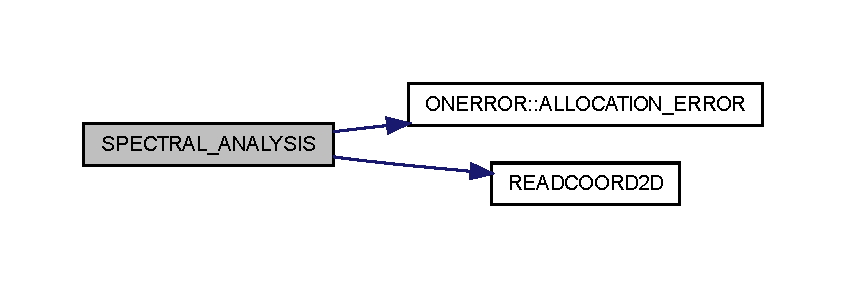
\includegraphics[width=400pt]{SPECTRAL__ANALYSIS_8f90_aa835ffe19690d8ed7c9292f4b331fd36_cgraph}
\end{center}
\end{figure}



\hypertarget{STATISTICS_8f90}{
\section{/home/fdietzsc/fortran/POSTPROC/SOURCES/STATISTICS.f90 File Reference}
\label{STATISTICS_8f90}\index{/home/fdietzsc/fortran/POSTPROC/SOURCES/STATISTICS.f90@{/home/fdietzsc/fortran/POSTPROC/SOURCES/STATISTICS.f90}}
}
\subsection*{Data Types}
\begin{DoxyCompactItemize}
\item 
interface \hyperlink{interfaceSTATISTICS_1_1MEAN}{STATISTICS::MEAN}
\item 
interface \hyperlink{interfaceSTATISTICS_1_1CORREL}{STATISTICS::CORREL}
\item 
interface \hyperlink{interfaceSTATISTICS_1_1SHIFT}{STATISTICS::SHIFT}
\item 
interface \hyperlink{interfaceSTATISTICS_1_1SPECTR}{STATISTICS::SPECTR}
\item 
interface \hyperlink{interfaceSTATISTICS_1_1DEVIAT}{STATISTICS::DEVIAT}
\end{DoxyCompactItemize}
\subsection*{Modules}
\begin{DoxyCompactItemize}
\item 
module \hyperlink{namespaceSTATISTICS}{STATISTICS}


\begin{DoxyCompactList}\small\item\em Provides functions for statistical computations. \end{DoxyCompactList}

\end{DoxyCompactItemize}
\subsection*{Functions/Subroutines}
\begin{DoxyCompactItemize}
\item 
subroutine \hyperlink{namespaceSTATISTICS_a4a3e7e4d1eb020e1128c01e60da55ead}{STATISTICS::SPEC2D} (IN1, IN2, NX, NY, OUT)
\begin{DoxyCompactList}\small\item\em Computes the three dimensional energy spectrum as the fourier transformation\par
 of the auto-\/correlation function. In the first step all three velocity\par
 components are fourier transformed. The second step consists of multiplying\par
 each transform with its conjugate complex in order to get the elements of the\par
 main diagonal of the velocity spectrum tensor \[\hat{R}_{ii}\left(\kappa,t\right)= \left<\hat{u}_i^{*}\left(\kappa,t\right)\,\hat{u}_i\left(\kappa,t\right)\right>= \Phi_{ii}\left(\kappa,t\right).\] After the components of $\Phi$ have been determined an integration over\par
 spherical shells has to be computed in order to get the three dimensional\par
 velocity spectrum. \[ E(k)=\oint\frac{1}{2}\Phi_{ii}(\kappa)\,d\mathrm{S}(\kappa) \] \end{DoxyCompactList}\item 
subroutine \hyperlink{namespaceSTATISTICS_abb792b2e62e57165b7e93764e07d1100}{STATISTICS::SPEC3D} (PROCNUM, IN1, IN2, IN3, NX, NY, NZ, OUT)
\begin{DoxyCompactList}\small\item\em Computes the three dimensional energy spectrum as the fourier transformation\par
 of the auto-\/correlation function. In the first step all three velocity\par
 components are fourier transformed. The second step consists of multiplying\par
 each transform with its conjugate complex in order to get the elements of the\par
 main diagonal of the velocity spectrum tensor \[\hat{R}_{ii}\left(\kappa,t\right)= \left<\hat{u}_i^{*}\left(\kappa,t\right)\,\hat{u}_i\left(\kappa,t\right)\right>= \Phi_{ii}\left(\kappa,t\right).\] After the components of $\Phi$ have been determined an integration over\par
 spherical shells has to be computed in order to get the three dimensional\par
 velocity spectrum. \[ E(k)=\oint\frac{1}{2}\Phi_{ii}(\kappa)\,d\mathrm{S}(\kappa) \] \end{DoxyCompactList}\item 
subroutine \hyperlink{namespaceSTATISTICS_a96f2830bd74ef7e612bb9b567a488fcb}{STATISTICS::DEVIATION} (VELO, NX, NY, NZ, SIGMA)
\begin{DoxyCompactList}\small\item\em Computes the standard deviation of the 3D input array. It is computed according to \[\sigma = \sqrt{\frac{1}{N} \sum_{i=1}^N (x_i - \mu)^2}, {\rm \ \ where\ \ } \mu = \frac{1}{N} \sum_{i=1}^N x_i. \] \end{DoxyCompactList}\item 
subroutine \hyperlink{namespaceSTATISTICS_ac51d5b789da17893b95107ddcb97813f}{STATISTICS::FFTSHIFT} (IN, NX, NY)
\begin{DoxyCompactList}\small\item\em Shifts the input array towards the zero frequencies. \end{DoxyCompactList}\item 
subroutine \hyperlink{namespaceSTATISTICS_a6631e38a843e8bfa986d426daebd6f4c}{STATISTICS::CORREL3D} (IN, NX, NY, NZ, OUT)
\begin{DoxyCompactList}\small\item\em Computes the auto-\/correlation coefficients of the 3D input array. The general definition of the auto-\/correlation (often exressed as the covariance) function is \[\mathrm{cov}(f,f)=\left(f\star f\right)(r)=\int_0^{\infty}f(x)\,f(x+r)\,dx \] One important feature of the correlation function is that is satisfies \[\mathcal{F}\{f\star f\}=(\mathcal{F}\{f\})^*\cdot\mathcal{F}\{f\}. \] In the code this allows for fast computations of the correlation function using the FFT approach. In order to get the correlation coefficients, the previously mentioned function has to be devided by standard deviations of the input arrays. \[r=\frac{\mathrm{cov}(f,f)}{\sigma_f\,\sigma_f} \] \end{DoxyCompactList}\item 
subroutine \hyperlink{namespaceSTATISTICS_a2529efc59bb06c5f2280df7277bf5c7d}{STATISTICS::XCORREL} (IN1, IN2, NX, NY, NZ, OUT)
\begin{DoxyCompactList}\small\item\em Computes the cross-\/correlation coefficients of the 3D input arrays. The general definition of the cross-\/correlation (often exressed as the covariance) function is \[\mathrm{cov}(f,g)=\left(f\star g\right)(r)=\int_0^{\infty}f(x)\,g(x+r)\,dx \] One important feature of the correlation function is that is satisfies \[\mathcal{F}\{f\star g\}=(\mathcal{F}\{f\})^*\cdot\mathcal{F}\{g\}. \] In the code this allows for fast computations of the correlation function using the FFT approach. In order to get the correlation coefficients, the previously mentioned function has to be devided by standard deviations of the input arrays. \[r=\frac{\mathrm{cov}(f,g)}{\sigma_f\,\sigma_g} \] Computes the cross-\/correlation of the 3D input array \end{DoxyCompactList}\item 
subroutine \hyperlink{namespaceSTATISTICS_a0e5d171eb0600a926c45883d16628bc5}{STATISTICS::MEAN1D} (M, NX)
\item 
subroutine \hyperlink{namespaceSTATISTICS_a95b82ef7e03a03d4b2ff850710558843}{STATISTICS::MEAN3D} (M, NX, NY, NZ, MEAN)
\begin{DoxyCompactList}\small\item\em Shifts the input array towards the zero frequencies. \end{DoxyCompactList}\item 
subroutine \hyperlink{namespaceSTATISTICS_a2e2608ba8eefb8af3541e4e9a09a6482}{STATISTICS::MEAN4D} (M, NX, NY, NZ, DIM, MEAN)
\end{DoxyCompactItemize}

\hypertarget{TIMER_8f90}{
\section{/home/fdietzsc/fortran/POSTPROC/SOURCES/TIMER.f90 File Reference}
\label{TIMER_8f90}\index{/home/fdietzsc/fortran/POSTPROC/SOURCES/TIMER.f90@{/home/fdietzsc/fortran/POSTPROC/SOURCES/TIMER.f90}}
}
\subsection*{Data Types}
\begin{DoxyCompactItemize}
\item 
type \hyperlink{typeTIMER__CLASS_1_1TIMER}{TIMER\_\-CLASS::TIMER}
\end{DoxyCompactItemize}
\subsection*{Modules}
\begin{DoxyCompactItemize}
\item 
module \hyperlink{namespaceTIMER__CLASS}{TIMER\_\-CLASS}
\end{DoxyCompactItemize}
\subsection*{Variables}
\begin{DoxyCompactItemize}
\item 
INTEGER, parameter \hyperlink{namespaceTIMER__CLASS_aad0658ec4217d15cb973a454db271c59}{TIMER\_\-CLASS::DBL} = SELECTED\_\-REAL\_\-KIND(p=DP)
\end{DoxyCompactItemize}

\printindex
\end{document}
